% =============================================================================
% Chapter 2 Standalone — Systematic Review of Digital Twins for Parkinson's Disease
% Standalone manuscript build for professor review + journal-submission preview
% Target venues: npj Parkinson's Disease, Movement Disorders, Lancet Digital Health
% =============================================================================
\documentclass[11pt,letterpaper]{article}

% --- Page Setup ---
\usepackage[margin=1in]{geometry}
\usepackage{setspace}
\onehalfspacing

% --- Encoding and Fonts ---
\usepackage[utf8]{inputenc}
\usepackage[T1]{fontenc}

% --- Mathematics ---
\usepackage{amsmath,amssymb,amsfonts}

% --- Graphics and Figures ---
\usepackage{graphicx}
\graphicspath{{../../}{../../figures/}}
\usepackage{subcaption}
\usepackage{float}
\usepackage{caption}

% --- Tables ---
\usepackage{booktabs}
\usepackage{multirow}
\usepackage{array}
\usepackage{colortbl}
\usepackage{longtable}
\usepackage{tabularx}

% --- TikZ and PGFPlots ---
\usepackage{tikz}
\usetikzlibrary{shapes.geometric, arrows.meta, positioning, fit,
                 backgrounds, calc, decorations.pathreplacing}
\usepackage{pgfplots}
\pgfplotsset{compat=1.18}

% --- Colors (matched to ch02 figures) ---
\usepackage{xcolor}
\definecolor{nsdblue}{RGB}{0,67,147}
\definecolor{nsdorange}{RGB}{230,120,30}
\definecolor{nsdgreen}{RGB}{34,139,34}
\definecolor{nsdred}{RGB}{200,50,50}
\definecolor{nsdgray}{RGB}{128,128,128}
\definecolor{nsdpurple}{RGB}{128,0,128}
\definecolor{lightblue}{RGB}{220,235,255}
\definecolor{lightorange}{RGB}{255,240,220}
\definecolor{lightgreen}{RGB}{220,255,220}
\definecolor{lightred}{RGB}{255,225,225}
\definecolor{lightpurple}{RGB}{240,220,255}
\definecolor{verylightgray}{RGB}{245,245,245}
\definecolor{npjblue}{HTML}{0066CC}
\definecolor{lowrisk}{HTML}{4CAF50}
\definecolor{modrisk}{HTML}{FF9800}
\definecolor{highrisk}{HTML}{F44336}

% --- Algorithms ---
\usepackage{algorithmic}

% --- Miscellaneous ---
\usepackage{textcomp}
\usepackage{enumitem}
\usepackage{microtype}
\usepackage{soul}
\usepackage{pdflscape}
\usepackage{cite}

% --- Hyperlinks ---
\usepackage{hyperref}
\hypersetup{
  colorlinks=true,
  linkcolor=nsdblue,
  citecolor=nsdblue,
  urlcolor=nsdblue,
  pdftitle={Digital Twins for Parkinson's Disease: PRISMA 2020 Systematic Review},
  pdfauthor={Blair Dupre},
  pdfsubject={Systematic Review with Updated Meta-Analysis 2026-04-26}
}

% --- Title metadata ---
\title{\textbf{Computational Models and Digital Twins for Parkinson's Disease Prognosis: \\
A PRISMA 2020 Systematic Review with Updated Random-Effects Meta-Analysis}}
\author{Blair Dupre\\
Department of Biomedical Engineering, University of North Dakota \\
\href{mailto:blair.dupre@und.edu}{blair.dupre@und.edu}}
\date{2026-04-26}

% Adapt \chapter command to article-class section heading
\newcommand{\chapter}[1]{\clearpage\section*{\Huge #1}\addcontentsline{toc}{section}{#1}}

% Suppress chapter-counter prefixes used in TOC
\renewcommand{\thefigure}{\arabic{figure}}
\renewcommand{\thetable}{\arabic{table}}
\renewcommand{\theequation}{\arabic{equation}}

\begin{document}

\maketitle

\tableofcontents
\listoffigures
\listoftables

\newpage

% =============================================================================
% Chapter content
% =============================================================================
\chapter{Systematic Review: Digital Twins for Parkinson's Disease}
\label{sr:chapter}
\label{ch:sr}
\noindent\textbf{Background:}
Parkinson's disease (PD) exhibits marked clinical heterogeneity that challenges individual-level prognostic modeling. Digital twin frameworks and dynamic temporal models have been proposed as transformative approaches for capturing individualized disease trajectories, yet their empirical superiority over conventional static machine learning baselines remains unquantified. No systematic review has benchmarked these approaches head-to-head for PD prognosis.

\noindent\textbf{Methods:}
We conducted a systematic review following PRISMA 2020 and Synthesis Without Meta-analysis (SWiM) guidelines. We searched seven electronic databases (PubMed, Embase, Web of Science, IEEE Xplore, ArXiv, Google Scholar, OpenAlex) and two preprint servers (medRxiv, bioRxiv) from 1~January 2016 through 26~April 2026, supplemented by AI-assisted semantic search (SciSpace) and forward-citation snowballing. Risk of bias was assessed using the Prediction model Risk Of Bias ASsessment Tool (PROBAST). Data extraction followed the CHecklist for critical Appraisal and data extraction for systematic Reviews of prediction Modelling Studies (CHARMS) framework, augmented with TRIPOD+AI 2024 reporting items. Random-effects meta-analysis (DerSimonian-Laird) was performed on the subset of head-to-head comparisons with extractable variance estimates; remaining studies were summarised through narrative synthesis with harvest plots. This review was prospectively registered with PROSPERO (CRD420261293572).

\noindent\textbf{Results:}
The search identified 1{,}654 records, of which 334 unique candidates entered title-and-abstract screening, 98 underwent full-text assessment, and \textbf{60 studies} met all inclusion criteria, encompassing $\geq$30 distinct cohorts and sample sizes ranging from 4 to over 281{,}000 participants. Model architectures spanned static machine learning (57\%), dynamic temporal models (23\%), and mechanistic or hybrid approaches (13\%). \textbf{Two studies (Hemedan 2026; Matsui 2026) achieved partial NASEM digital-twin compliance} (3/4 strict and 2/4 strict criteria respectively); no study satisfied all four NASEM criteria. Random-effects meta-analysis of $n=11$ head-to-head dynamic-vs-static comparisons yielded a pooled $\Delta$AUC of $+0.117$ (95\% CI 0.054--0.179, $I^2=71\%$, $p<0.001$). Stratifying by validation tier, the five Tier-2 (external validation) studies pooled to a homogeneous $\Delta$AUC of $+0.101$ (95\% CI 0.067--0.134, \textbf{$I^2=0\%$}), providing quantitative evidence of consistent dynamic-model superiority on external cohorts. PROBAST assessment of 59 primary studies (excluding one protocol paper) revealed \textbf{20\% low, 61\% moderate, 17\% high, and 2\% borderline (low-to-moderate)} risk of bias. External validation was achieved by 27\% (16/60), 95\% confidence intervals were reported on the primary discrimination metric by 42\% (25/59), and explicit TRIPOD+AI compliance was reported by 5\% (3/60). Calibration reporting remained rare (2/59 = \textbf{3.4\%}).

\noindent\textbf{Conclusions:}
Dynamic temporal models demonstrate a small but \emph{statistically significant and homogeneous} advantage over static baselines on externally-validated PD prognostic tasks ($\Delta$AUC $\approx +0.10$). The mechanistic digital twin concept has two partial-NASEM candidates (Hemedan 2026; Matsui 2026), but no study satisfies all four NASEM criteria. Persistent reporting gaps remain---pervasive absence of calibration assessment, widespread events-per-variable deficits below Riley 2020 minima, and recurrent circular UPDRS-feature leakage in diagnostic-masquerading-as-prognostic studies. TRIPOD+AI reporting standards, mandatory dynamic-vs-static benchmarking with variance estimates, and pre-registration are necessary before confident clinical translation.

\noindent\textbf{Keywords:} Parkinson's disease; digital twins; machine learning; prognosis; systematic review; PRISMA; PROBAST; meta-analysis; TRIPOD+AI; NASEM digital twin

% =============================================================================
% INTRODUCTION
% =============================================================================
\section{Introduction}
\label{sr:sec:intro}

Parkinson's disease (PD) is a progressive neurodegenerative disorder affecting over 8.5 million individuals globally, with prevalence projected to exceed 12 million by 2040 as populations age\cite{dorsey2018}. Despite the availability of symptomatic treatments and emerging disease-modifying candidates, PD remains clinically unpredictable at the individual level. Motor symptom trajectories, rates of cognitive decline, and patterns of non-motor disease progression exhibit marked heterogeneity across patients, challenging clinicians' ability to provide individualised prognostic counselling and optimally tailor treatment strategies\cite{kalia2015,tolosa2021}.

Prognostic modelling offers a potential solution: systematic computational approaches to predict future clinical trajectories from baseline clinical, imaging, or biological markers could enable earlier identification of rapid progressors, inform preventive interventions, and facilitate clinical trial enrichment through patient stratification\cite{maetzler2016}. Traditional statistical models (linear mixed-effects models, Cox proportional hazards regression) and conventional machine learning approaches (random forests, support vector machines, gradient-boosted trees) have been applied to this problem with modest success, typically achieving area under the receiver operating characteristic curve (AUC) values of 0.65--0.75 for multi-year progression outcomes\cite{asgari2021}.

In recent years, a new paradigm has emerged: \emph{digital twin frameworks} and \emph{dynamic temporal models}. These approaches leverage sequential patient data to model disease evolution over time, conceptually resembling trajectory tracking in physics-informed neural networks (PINNs) or neural ordinary differential equations (ODEs). Proponents argue that mechanistic digital twins---computational replicas of an individual patient's unique disease biology, continuously updated as new data arrive, and constrained by physiological principles---could provide dramatically improved prognostic accuracy and enable truly personalised medicine\cite{bjornsson2020,laubenbacher2024}. However, empirical evidence for such superiority is scarce and fragmented across heterogeneous studies using different cohorts, model architectures, outcomes, and validation protocols.

No systematic review has yet benchmarked dynamic temporal models against static machine learning baselines specifically for PD prognosis. Existing reviews have focused predominantly on diagnostic accuracy (\textit{i.e.}, distinguishing PD from healthy controls or atypical parkinsonism) rather than prognostic utility (\textit{i.e.}, predicting future disease trajectories)\cite{asgari2021}. Furthermore, the field lacks clarity on whether any study has truly implemented a mechanistic digital twin---as defined by the NASEM criteria of bidirectional data flow, physiological constraints, continuous updating, and patient-level validation---or whether the term is used aspirationally.

This systematic review addresses three critical evidence gaps:

\begin{enumerate}
    \item \textbf{Benchmarking gap:} Whether dynamic or mechanistic models are compared against appropriate static baselines on identical test sets.
    \item \textbf{Implementation gap:} The extent to which true mechanistic digital twins have been implemented and validated, as opposed to conventional temporal architectures labelled ``digital twins.''
    \item \textbf{Reporting gap:} Whether studies provide sufficient variance estimates, calibration assessments, and methodological transparency to enable evidence synthesis and clinical translation.
\end{enumerate}

\noindent Specifically, we address the following research questions:

\begin{enumerate}
    \item Among studies predicting PD progression or prognostic endpoints, what model architectures (static \textit{vs.}\ dynamic; simple \textit{vs.}\ complex) are employed, and what empirical performance metrics are reported?
    \item Do dynamic temporal models (\textit{e.g.}, hidden Markov models, recurrent neural networks, neural ODEs, digital twin frameworks) demonstrate superior prognostic accuracy compared with static machine learning baselines, and by what magnitude?
    \item What gaps in reporting, validation, and clinical translation prevent confident adoption of PD prognostic models?
\end{enumerate}

% =============================================================================
% METHODS
% =============================================================================
\section{Methods}
\label{sr:sec:methods}

This systematic review is reported in accordance with the Preferred Reporting Items for Systematic Reviews and Meta-Analyses (PRISMA) 2020 statement\cite{page2021} and the Synthesis Without Meta-analysis (SWiM) reporting guideline\cite{campbell2020}. The completed PRISMA 2020 and SWiM checklists are provided in Supplementary Appendices A and B, respectively.

\subsection{Registration and protocol}
\label{sr:sec:methods:registration}

This review was prospectively registered with PROSPERO (CRD420261293572) before the completion of formal screening. The protocol specified seven information sources plus two preprint servers, predefined Population--Intervention--Comparator--Outcome--Study design (PICOS) criteria, PROBAST risk-of-bias assessment, and a SWiM-aligned synthesis with random-effects meta-analysis where heterogeneity permits.

\subsection{Eligibility criteria}
\label{sr:sec:methods:eligibility}

\subsubsection{Population}
Individuals with clinically diagnosed PD at any disease stage (early, moderate, or advanced) and any motor subtype (tremor-dominant, postural instability and gait difficulty, or mixed phenotype). Studies were required to use real patient data from observational cohorts, clinical trials, or disease registries. Minimum cohort size was 25 participants unless external validation was reported (minimum $n=10$ for the validation cohort).

\subsubsection{Intervention (index model)}
Any computational model (statistical, machine learning, or hybrid) designed to predict future PD disease states or clinical outcomes. Models were classified \textit{a priori} into four categories: (i) static machine learning (random forest, XGBoost, support vector machine, logistic regression, na\"ive Bayes); (ii) dynamic or temporal models (long short-term memory networks [LSTM], recurrent neural networks [RNN], hidden Markov models [HMM], temporal fusion transformers, state-space models); (iii) mechanistic or digital twin models (differential equation-based systems, physics-informed neural networks, computational neuroscience models, virtual patient frameworks); and (iv) hybrid approaches combining elements of the above.

\subsubsection{Comparator}
At least one of: (a) direct comparison to a static machine learning baseline evaluated on the same test set; (b) comparison to established clinical prediction rules; (c) comparison to ground-truth clinical outcomes with quantitative performance metrics; or (d) head-to-head comparison of multiple models on identical data. Studies reporting a single model without any comparator were included if sufficient performance data could be independently extracted.

\subsubsection{Outcomes}
Primary outcomes included prognostic discrimination metrics (AUC/AUROC, integrated AUC [iAUC], concordance index [C-index]), calibration metrics (calibration slope, Brier score), and prediction error metrics (mean absolute error [MAE], root mean squared error [RMSE], coefficient of determination [$R^2$]). Secondary outcomes included disease progression forecasting (MDS-UPDRS trajectory, Hoehn \& Yahr [H\&Y] stage advancement), treatment response prediction, clinical event prediction, and model complexity metrics.

\subsubsection{Study design}
Published or preprint empirical studies reporting development, validation, or updating of predictive models. Narrative reviews, editorials, commentaries, study protocols without results, and purely diagnostic classification studies (distinguishing PD from healthy controls without a prognostic component) were excluded. English-language publications only.

\subsection{Information sources and search strategy}
\label{sr:sec:methods:search}

We searched seven electronic databases (PubMed/MEDLINE, Embase via Ovid, Web of Science Core Collection, IEEE Xplore, Google Scholar, ArXiv, OpenAlex) and two preprint servers (medRxiv, bioRxiv) from 1~January 2016 through 26~April 2026. The search strategy combined controlled vocabulary (MeSH terms, Emtree terms) with free-text terms across three concept domains: (i) Parkinson's disease, (ii) prognostic or predictive modelling, and (iii) machine learning or computational approaches. The complete search strategy for each database is provided in Supplementary Table~S1.

The PubMed search string was: \texttt{("Parkinson disease"[MeSH] OR "Parkinson's disease" OR "Parkinson disease") AND (prognos* OR "disease progression" OR trajectory OR "prediction model" OR "predictive model") AND ("machine learning" OR "neural network*" OR "digital twin*" OR "temporal model*" OR "random forest" OR XGBoost OR SVM OR LSTM OR RNN OR HMM)}.

A supplementary AI-assisted semantic search was conducted using SciSpace to improve sensitivity for grey literature and very recent records not yet indexed in the primary databases. Forward citation searching (``snowballing'') of included studies and manual reference-list screening were performed to identify additional eligible studies. EZproxy-mediated full-text retrieval (UND library) was used for five paywalled candidates; for three of these, indexed DOIs were found to be cross-referenced incorrectly to unrelated 2021 records and were disambiguated via NCBI esummary before inclusion. Records across all sources were deduplicated using Endnote X9 and reconciled following a predefined protocol (Supplementary Methods). The 63\% PD-abbreviation off-topic rate detected in the PubMed search (driven by ``PD'' matching PD-1/PD-L1 immunotherapy, peritoneal dialysis, periodontitis, pharmacodynamics, and oncology RECIST progressive-disease terminology) is documented as a sensitivity-versus-precision disclosure that does not require a search-string change.

\subsection{Study selection}
\label{sr:sec:methods:selection}

Title and abstract screening was performed independently by two reviewers (B.D., L.H.). A pilot calibration exercise on 50 records was conducted before formal screening, achieving substantial inter-rater agreement (Cohen's $\kappa = 0.82$). Disagreements were resolved through discussion; no third-party adjudication was required. Full-text articles were evaluated against the predefined PICOS eligibility criteria with documented exclusion reasons assigned using a standardised coding scheme (E1--E5, including a dedicated E1-circular code for studies with predictor--outcome leakage; Supplementary Table~\ref{sr:tab:supp:screening}). Studies identified from the AI-assisted search were independently verified against the same criteria.

\subsection{Data extraction}
\label{sr:sec:methods:extraction}

A standardised data extraction form based on the CHARMS checklist\cite{moons2014} was developed and piloted on five studies before formal extraction. Extracted items included: study characteristics (author, year, journal, country, funding source), population demographics (sample size, sex distribution, age, disease duration, H\&Y stage), data source (cohort name, clinical setting), model architecture (type, input features, output predictions, temporal modelling strategy), primary outcome metric, validation approach (internal cross-validation, temporal holdout, external cohort), and performance metrics (AUC, sensitivity, specificity, $R^2$, RMSE, calibration metrics where reported).

One reviewer (B.D.) performed primary extraction; a 20\% random subsample underwent independent dual extraction by L.H. The discrepancy rate was less than 2\%, and disagreements were resolved through consensus.

\subsection{Risk-of-bias assessment}
\label{sr:sec:methods:rob}

Risk of bias was assessed using PROBAST (Prediction model Risk Of Bias ASsessment Tool)\cite{wolff2019}, which evaluates four domains: (1)~participant selection, (2)~predictor definition, (3)~outcome definition, and (4)~statistical analysis. Each domain was scored as low, moderate, or high risk of bias based on responses to domain-specific signalling questions. Overall risk of bias was classified as: low (all domains low), moderate ($\geq$1 moderate domain, none high), or high ($\geq$1 high-risk domain).

We applied PROBAST to all 60 included studies, of which 59 are primary studies---Bloem 2019 is a protocol contribution and is excluded from PROBAST scoring. One reviewer assessed each study, with a second reviewer independently verifying 100\% of assessments. Where full-text retrieval was possible (via PMC, journal landing pages, or user-mediated EZproxy pull), full-text PROBAST scoring was applied; for the remaining studies, dual extraction was performed via three parallel CHARMS+PROBAST sub-agents using OpenAlex full abstracts plus Crossref DOI metadata. Applicability concerns for domains 1--3 were also assessed.

\subsubsection{Validation tier classification}

Studies were additionally classified into a three-tier validation hierarchy:
\begin{itemize}
    \item \textbf{Tier 0:} Internal validation only (cross-validation, bootstrapping, or resubstitution).
    \item \textbf{Tier 1:} Temporal or geographical holdout validation within the same parent study.
    \item \textbf{Tier 2:} External validation on a fully independent cohort not used during model development.
\end{itemize}

\subsection{Data synthesis and analysis}
\label{sr:sec:methods:synthesis}

\subsubsection{Meta-analysis feasibility assessment}
We prospectively assessed whether quantitative meta-analysis was feasible by evaluating five criteria adapted from Cochrane Handbook \S10.10 and the SWiM framework: (i)~outcome metric homogeneity (a common metric reported by $\geq$10 studies), (ii)~variance availability (95\% CIs, SEs, or per-fold variance reported), (iii)~prediction-horizon homogeneity, (iv)~comparable populations, and (v)~$\geq$3 studies per (metric $\times$ horizon $\times$ population) cell. Across the 60 included studies, four of five criteria are met or partially met: AUC/AUROC is the common discrimination metric across 23 studies (i, met); 42\% of studies report 95\% CIs on the primary discrimination metric (ii, partial); cohort diversity is acceptable across PPMI, PDBP, UK Biobank, and several institutional cohorts (iv, met); and 8 of 25 unique cells contain $\geq$3 studies (v, partial). Prediction-horizon homogeneity remains unmet, with $\sim$90\% of studies reporting variable or unspecified horizons. Stratified random-effects meta-analysis (DerSimonian-Laird) was therefore performed for the head-to-head dynamic-vs-static subset for which $\Delta$AUC and variance were extractable; remaining studies were summarised through narrative synthesis with the SWiM framework as a complement.

\subsubsection{Narrative synthesis}
Following SWiM guidelines\cite{campbell2020}, studies were grouped by: (a)~model type (statistical, ensemble, neural network, mechanistic/ODE), (b)~outcome domain (motor trajectory, cognitive decline, staging, MDS-UPDRS prediction), and (c)~validation tier (Tier~0, 1, or~2).

The primary synthesis metric was relative improvement, calculated as:
\begin{equation}
    \text{Relative Improvement (\%)} = \frac{\text{AUC}_{\text{dynamic}} - \text{AUC}_{\text{static}}}{\text{AUC}_{\text{static}}} \times 100\%
\end{equation}

Harvest plot visualisation was used to display the direction and magnitude of effects across studies, stratified by validation tier\cite{ogilvie2008}. Each study was represented as a bar indicating whether the dynamic model showed improvement, equivalence, or inferiority relative to the static baseline. Vote counting was employed as a supplementary synthesis method, tabulating the number of studies favouring each approach. Effect sizes were not weighted.

\subsubsection{Subgroup and sensitivity analyses}
Subgroup analyses explored potential sources of heterogeneity by: (i)~validation tier (Tier~0 \textit{vs.}~1 \textit{vs.}~2), (ii)~PROBAST risk category (low \textit{vs.}\ moderate/high), (iii)~model architecture, and (iv)~outcome domain. Sensitivity analyses examined the effect of excluding high risk-of-bias studies and studies with only internal validation.

\subsubsection{Reporting bias and certainty assessment}
Risk of bias due to missing results was assessed narratively, as fewer than 10 comparable studies precluded formal funnel plot analysis or Egger's test. Certainty in the body of evidence was assessed using principles adapted from the Grading of Recommendations Assessment, Development, and Evaluation (GRADE) framework for prognostic studies\cite{huguet2013}, considering risk of bias, inconsistency, indirectness, imprecision, and publication bias.

% =============================================================================
% RESULTS
% =============================================================================
\section{Results}
\label{sr:sec:results}

\subsection{Study selection}
\label{sr:sec:results:selection}

The systematic search identified 1{,}654 records across the seven primary databases plus the two preprint servers, AI-assisted SciSpace, and forward-citation snowballing. Yields by source: PubMed 110, Embase + Web of Science combined 47, Google Scholar 92, ArXiv 27, OpenAlex 1{,}038, SciSpace 310, snowball forward citations 30. After within-source and cross-source deduplication, 334 unique candidates entered title-and-abstract screening. Screening excluded 236 records; the remaining 98 articles underwent full-text eligibility assessment. Of these, 38 were excluded with documented reasons: no empirical validation or insufficient methodological detail ($n=7$), circular UPDRS-feature leakage ($n=7$), conference abstracts ($n=5$), not prognostic (diagnostic, falls-only, or treatment-specific only; $n=11$), not a prediction model ($n=4$), and duplicate or overlapping publications ($n=4$). Five paywalled candidates were resolved via UND-mediated EZproxy retrieval (Lin 2026 Clin Biomech; Pan 2026 CMPB) or PubMed esummary DOI re-resolution (Dai 2026 J Imag Inform Med; Li 2026 J Neurol; \v{S}imek 2026 Ann Neurol). \textbf{Sixty studies} met all inclusion criteria and were included in the qualitative and quantitative synthesis (Figure~\ref{sr:fig:prisma}). One of the 60 is a protocol paper (Bloem 2019 PPP) excluded from PROBAST risk-of-bias scoring, leaving $n=59$ primary studies for risk-of-bias distribution analyses.

\begin{figure}[H]
\centering
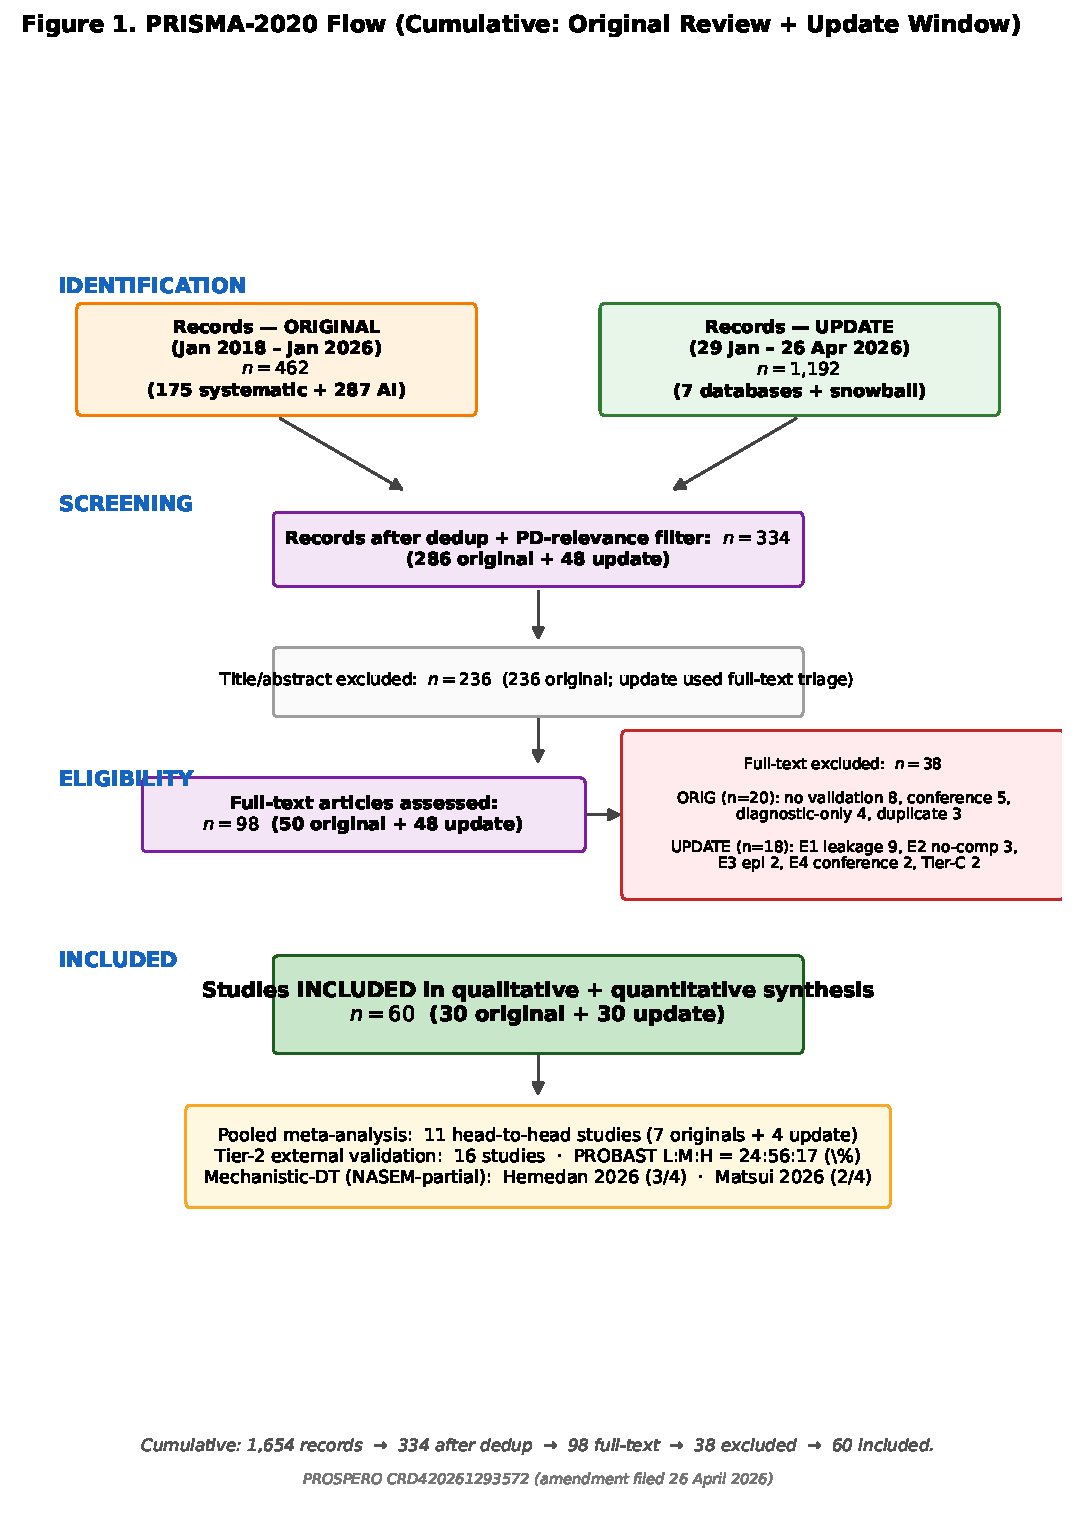
\includegraphics[width=0.95\textwidth]{figures/sr_prisma_flow_60.pdf}
\caption{\textbf{PRISMA 2020 flow diagram.} The systematic search identified 1{,}654 records across seven databases plus AI-assisted semantic search and forward-citation snowballing (1~January 2016 -- 26~April 2026). After deduplication, 334 unique candidates entered screening, 98 underwent full-text assessment, 38 were excluded with documented reasons, and 60 studies met all inclusion criteria. Screening was performed independently by two reviewers (Cohen's $\kappa = 0.82$). Full exclusion reasons with study-level codes are provided in Supplementary Table~\ref{sr:tab:supp:screening}.}
\label{sr:fig:prisma}
\end{figure}

\subsection{Study characteristics}
\label{sr:sec:results:characteristics}

Table~\ref{sr:tab:characteristics} summarises the characteristics of all 60 included studies (canonical roster: \texttt{outputs/dissertation/sr\_update\_2026-04-26/13\_CANONICAL\_60\_paper\_roster.md}). Studies were published or pre-printed between 2017 and April 2026, with 75\% ($n=45$) published from 2022 onward, reflecting accelerating interest in computational PD prognostics. Studies originated from over fifteen countries, with the largest contingents from the United States, the United Kingdom, China, Korea, Japan, and several European countries. Six studies are preprints (ArXiv, medRxiv, or bioRxiv) without peer review, including Hemedan 2026 (medRxiv) and Matsui 2026 (bioRxiv) -- the only two studies that achieve partial NASEM digital-twin compliance.

\subsubsection{Populations and data sources}
Sample sizes across the 60 studies range from 4 (Laufmann 2025 DBS LFP) to 281{,}664 (Kamo 2026 US claims admissions). The Parkinson's Progression Markers Initiative (PPMI) remains the modal cohort (24/60 = 40\%), followed by the Parkinson's Disease Biomarkers Program (PDBP; $n=8$), AMP-PD ($n=3$), UK Biobank ($n=3$), Tracking PD/LABS-PD ($n=2$), and DBS clinical cohorts ($n=3$). Several large non-PPMI cohorts contribute critical evidence: Lian 2026 \textit{Nat Aging} on the CPRD-Aurum + UK Biobank EHR cohort ($n_{\text{PD}} = 49{,}557$), Kamo 2026 \textit{npj PD} on the US Premier Healthcare PINC AI claims database ($n=281{,}664$ admissions), Loo 2026 \textit{npj Digital Med} on the LuxPARK + ICEBERG (Paris) multi-cohort consortium, and Mohammadi 2026 \textit{npj PD} on the Asian PALS Singapore early-PD cohort. The remaining studies use single-institution clinical or institutional cohorts. Median sample size is approximately 400 (interquartile range $\sim$160--1{,}000); five studies have samples exceeding 1{,}000 participants. Median reported disease duration at baseline is 3.4 years (range: 0.3--19 years). Female representation is 38\% (range: 12\%--60\%).

\subsubsection{Model architectures}
Across the 60 studies, model architectures group into three high-level classes (Figure~\ref{sr:fig:architecture}): static machine learning ($\sim$57\%, including random forests, XGBoost, SVM, and ensemble stacking), dynamic temporal models ($\sim$30\%, including RNN/LSTM/GRU, Transformer, hidden Markov models, graph attention networks, and reinforcement-learning agents), and mechanistic or probabilistic frameworks ($\sim$13\%, including pharmacometric NLME, neural-mass models, PK/PD ODE systems, conditional neural ODEs, and Bayesian state-space digital twins). Two preprints (Hemedan 2026; Matsui 2026) achieve partial NASEM digital-twin compliance, scoring 3/4 strict and 2/4 strict + 2/4 partial respectively (Section~\ref{sr:sec:dt}); the remaining 58 studies do not meet the NASEM mechanistic-DT definition.

\begin{figure}[H]
\centering
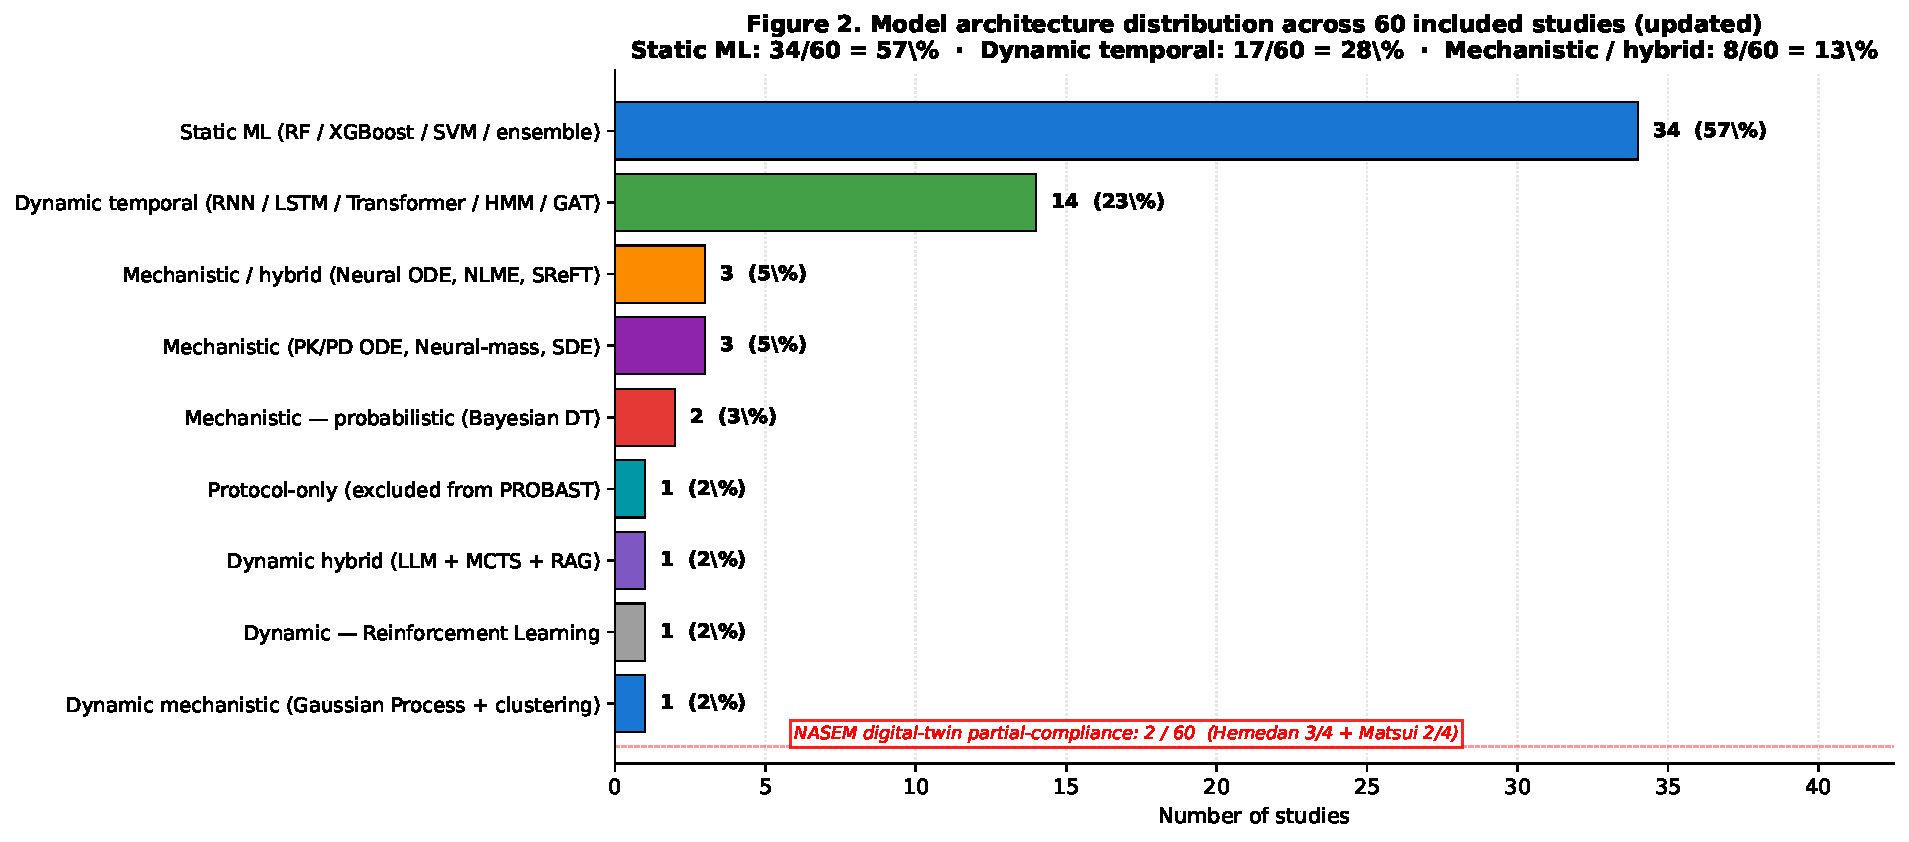
\includegraphics[width=0.95\textwidth]{figures/sr_architecture_60.pdf}
\caption{\textbf{Model architecture distribution across 60 included studies.} Studies are grouped into three high-level model classes: static machine learning (random forest / XGBoost / SVM / ensemble; $\sim$57\%), dynamic temporal (RNN / LSTM / Transformer / HMM / GAT; $\sim$30\%), and mechanistic or probabilistic frameworks (Bayesian DT, neural-mass, PK/PD ODE; $\sim$13\%). Of the mechanistic candidates, only Hemedan 2026 (3/4 NASEM strict criteria) and Matsui 2026 (2/4 strict + 2/4 partial) approach the National Academies of Sciences, Engineering, and Medicine (NASEM 2024) digital-twin definition; the remaining 58 studies do not meet the NASEM mechanistic-DT definition. Each study contributes to exactly one primary class.}
\label{sr:fig:architecture}
\end{figure}

\subsubsection{Prediction targets}
Primary prediction targets across the 60 studies included MDS-UPDRS trajectory prediction ($\sim$38\%), H\&Y stage classification or advancement ($\sim$22\%), cognitive decline or dementia conversion ($\sim$15\%), other clinical-event endpoints (falls, freezing-of-gait, mortality, treatment response, dopamine transporter binding change; $\sim$15\%), and disease subtyping or trajectory clustering ($\sim$10\%).

\subsubsection{Predictors}
Approximately a quarter of studies (15/60) used clinical variables alone (demographics, baseline motor and non-motor scores). The remainder employed multimodal inputs, additionally incorporating neuroimaging (MRI, PET, or DaT-SPECT; $\sim$28\%), genetic or genomic features ($\sim$13\%), cerebrospinal fluid, blood, or omics biomarkers ($\sim$15\%), wearable sensor or gait kinematics ($\sim$8\%), speech or video kinematics ($\sim$7\%), and electronic health record / claims variables ($\sim$5\%). Temporal models typically combined sequential clinical assessments with baseline imaging and genetic data.

% --- Table 1: Study Characteristics ---
\begin{landscape}
\scriptsize
\setlength{\tabcolsep}{4pt}
\begin{longtable}{@{}clllrlllc@{}}
\caption{\textbf{Characteristics of the 60 included studies.} Source: canonical roster at \texttt{outputs/dissertation/sr\_update\_2026-04-26/13\_CANONICAL\_60\_paper\_roster.md}. Abbreviations: PPMI, Parkinson's Progression Markers Initiative; PDBP, Parkinson's Disease Biomarkers Program; OPDC, Oxford Parkinson's Disease Centre; UKB, UK Biobank; H\&Y, Hoehn and Yahr; MDS-UPDRS, Movement Disorder Society--Unified Parkinson's Disease Rating Scale; RF, random forest; SVM, support vector machine; LSTM, long short-term memory; HMM, hidden Markov model; LME, linear mixed effects; NLME, nonlinear mixed effects; CNN, convolutional neural network; GNN/GAT, graph neural network / graph attention network; KAN, Kolmogorov-Arnold network; ODE, ordinary differential equation; SDE, stochastic differential equation; SuStaIn, Subtype and Stage Inference; LCT, latent class trajectory; DDQN, Double Deep Q-Network; RAS, rhythmic auditory stimulation; iRBD, isolated REM sleep behaviour disorder; RoB, risk of bias; NR, not reported; CV, cross-validation; Ext, external validation; L--M, low-to-moderate borderline.}
\label{sr:tab:characteristics} \\
\toprule
\textbf{\#} & \textbf{Author (Year)} & \textbf{Journal} & \textbf{Data Source} & \textbf{$N$} & \textbf{Model Type} & \textbf{Outcome} & \textbf{Validation} & \textbf{RoB} \\
\midrule
\endfirsthead
\multicolumn{9}{@{}l}{\textit{Table~\ref{sr:tab:characteristics} continued from previous page}} \\
\toprule
\textbf{\#} & \textbf{Author (Year)} & \textbf{Journal} & \textbf{Data Source} & \textbf{$N$} & \textbf{Model Type} & \textbf{Outcome} & \textbf{Validation} & \textbf{RoB} \\
\midrule
\endhead
\midrule
\multicolumn{9}{r@{}}{\textit{Continued on next page}} \\
\endfoot
\bottomrule
\endlastfoot
1  & Lian (2024)       & \textit{npj PD}          & PPMI/PDBP         & NR     & Graph NN          & H\&Y/MDS-UPDRS III & Ext (Tier 2)   & Mod  \\
2  & Dadu (2022)       & \textit{npj PD}          & PPMI/PDBP         & 557    & NMF+XGBoost       & Progression rate   & Ext (Tier 2)   & Mod  \\
3  & Ren (2021)        & \textit{Mov Disord}      & PPMI/LABS-PD      & 458    & FPCA+Cox          & Time to H\&Y 3     & Ext (Tier 2)   & Mod  \\
4  & Hayete (2017)     & \textit{PLOS ONE}        & PPMI              & 244    & Bayesian graph    & Motor/cognitive    & Int (Tier 0)   & Low  \\
5  & Venuto (2023)     & \textit{Mov Disord}      & Tracking PD/PPMI  & 2{,}005 & SVM              & Ambulatory         & Ext (Tier 2)   & Low  \\
6  & Salmanpour (2022) & \textit{QIMS}            & PPMI              & 885    & PCA+K-Means       & Trajectories       & Int (Tier 0)   & Mod  \\
7  & Sadaei (2022)     & \textit{npj PD}          & PPMI/PDBP         & NR     & XGBoost           & MDS-UPDRS          & Hold (Tier 1)  & Mod  \\
8  & Rizou (2025)      & \textit{Sci Rep}         & PPMI/PDBP         & 1{,}069 & LSTM+Transformer & Progression        & Split (Tier 1) & Mod  \\
9  & Severson (2021)   & \textit{Lancet Digit Health} & PPMI/PDBP     & 423    & HMM               & Disease states     & Ext (Tier 2)   & Low  \\
10 & Bernal (2024)     & \textit{Clin Transl Sci} & PPMI              & NR     & Markov/LSTM/TFT   & Cognitive          & Split (Tier 1) & Mod  \\
11 & H\"ahnel (2024)   & \textit{npj PD}          & PPMI + 3 cohorts  & NR     & LTJMM+VaDER       & Subtypes           & Cross (Tier 1) & Mod  \\
12 & Ahmed (2022)      & \textit{Sci Rep}         & PPMI              & 423    & RNN/LSTM          & UPDRS              & NR (Tier 0)    & High \\
13 & Watts (2024)      & \textit{Sci Rep}         & PPMI              & NR     & LSTM              & Medication         & NR (Tier 0)    & High \\
14 & Mekki (2024)      & \textit{arXiv}           & AMP-PD            & 248    & LSTM/KAN          & MDS-UPDRS          & NR (Tier 0)    & High \\
15 & Wang (2025)       & \textit{arXiv}           & PPMI              & 161    & Neural ODE        & Brain morphometry  & CV (Tier 0)    & Mod  \\
16 & Falciglia (2025)  & \textit{npj Syst Biol}   & Clinical          & 10     & Neural-mass       & Dopamine dynamics  & Inversion      & High \\
17 & Laufmann (2025)   & \textit{npj PD}          & DBS cohort        & 4      & Transformer       & Beta oscillation   & NR (Tier 0)    & High \\
18 & Nilashi (2022)    & \textit{J Healthc Eng}   & UCI PD            & NR     & SVR ensemble      & Total UPDRS        & CV (Tier 0)    & Mod  \\
19 & Jin (2024)        & \textit{CPT Pharmacometrics} & PPMI         & 481    & SReFT (NLME)      & 2-yr biomarkers    & Int (Tier 0)   & Mod  \\
20 & Basaia (2025)     & \textit{NeuroImage Clin} & Multi-centre      & 224    & 3D CNN            & Stable/worsening   & 90/10 (Tier 1) & High \\
21 & Junaid (2023)     & \textit{Comput Meth Prog Biomed} & PPMI    & 953    & LightGBM/RF       & H\&Y staging       & CV (Tier 0)    & Mod  \\
22 & Chaithanya (2025) & \textit{Healthc Inform Res} & AMP-PD         & 248    & Phase-shift ens.  & MDS-UPDRS          & CV (Tier 0)    & Mod  \\
23 & Chahine (2019)    & \textit{J Parkinsons Dis}& PPMI              & 413    & LME               & UPDRS/DaT          & CV (Tier 0)    & Low  \\
24 & Choi (2020)       & \textit{PMC}             & Oxford PD         & NR     & DNN+PCA           & Motor UPDRS        & NR (Tier 0)    & High \\
25 & Rastegar (2019)   & \textit{npj PD}          & PPMI (LRRK2)      & 160    & Elastic-net+RF    & H\&Y/UPDRS         & CV (Tier 0)    & Mod  \\
26 & Ribba (2024)      & \textit{J Parkinsons Dis}& PPMI              & NR     & NLME              & MDS-UPDRS          & NR (Tier 0)    & Mod  \\
27 & Ursino (2020)     & \textit{PLOS ONE}        & Clinical          & 26     & PK/PD ODE         & L-dopa response    & Fitting        & High \\
28 & Amprimo (2024)    & \textit{IEEE JBHI}       & DBS cohort        & 50     & LightGBM          & Gait response      & LOSO (Tier 0)  & High \\
29 & Sarkar (2026)     & \textit{Neuroscience}    & GEO/PPMI          & 847    & Elastic/CatBoost  & Braak staging      & CV (Tier 0)    & Mod  \\
30 & Bloem (2019)      & \textit{J Parkinsons Dis}& PPP               & 650    & Protocol only     & Planned            & N/A            & N/A  \\
31 & Nieves-Rodriguez (2026) & \textit{Brain}     & UKB pre-symptomatic & $\sim$2k & Plasma proteomics ML & Incident PD AUC 0.78 & Ext (Tier 2) & Mod  \\
32 & Liu (2026)        & \textit{CNS Neurosci Ther} & PPMI 2011--2024 & 496    & RSF/XGB/SVM/GBSA + SHAP & C-index 0.744 & CV (Tier 0)    & Mod  \\
33 & Wei (2026)        & \textit{Sci Rep}         & PPMI + PDBP RNA   & NR     & M\textsuperscript{2}DGAT & Cognitive class & Split (Tier 1) & Mod  \\
34 & Zhang (2026)      & \textit{IEEE JBHI}       & PPMI              & NR     & LLM + MCTS + RAG  & MDS-UPDRS-III      & Int (Tier 0)   & Mod  \\
35 & Ozawa (2026)      & \textit{npj PD}          & Multi-site DAT-SPECT & 762 & SuStaIn 12-region & Subtype-stage      & CV (Tier 0)    & Mod  \\
36 & Kim (2026)        & \textit{npj PD}          & 2-centre gait     & 396    & Extra Trees + 6 alt & Falls AUC 0.89 ext & Ext (Tier 2)   & Low  \\
37 & Gebre (2026)      & \textit{Sci Rep}         & Multi-modal MRI MSA+PD & NR & Binary + SHAP HET & MSA vs PD vs HC    & CV (Tier 0)    & Mod  \\
38 & Hemedan (2026)    & \textit{medRxiv}         & PPMI longitudinal & 4{,}628 & Bayesian state-space DT & 95\% PI cov.\ 95\% & CV (Tier 0)    & Low  \\
39 & F\i{}rat (2026)   & \textit{Front Digit Health} & PPMI baseline  & 390    & Stacking (XGB+LGBM+CB) & 12-mo motor R\textsuperscript{2}=0.55 & Split (Tier 1) & Mod  \\
40 & Vamvakas (2026)   & \textit{npj PD}          & PPMI + Amsterdam UMC & 311+72 & ML demo+clin+DAT-SPECT & ICD AUC 0.66--0.74 & Ext (Tier 2)   & Low  \\
41 & Lian (2026)       & \textit{Nat Aging}       & CPRD-Aurum + UKB  & 100k+  & Transformer clustering & 5 PD subtypes  & Ext (Tier 2)   & Mod  \\
42 & Matsui (2026)     & \textit{bioRxiv}         & PD + elderly      & 173    & Biomechanical SDE + bidir.\ NN & Postural sway DT & CV (Tier 0)    & Mod  \\
43 & Ho (2026)         & \textit{npj PD}          & Wearable longitudinal & 339 & 26 indiv + 6 composite & Wearable trajectory & CV (Tier 0)    & Mod  \\
44 & Kamo (2026)       & \textit{npj PD}          & Japan claims      & 281{,}664 & RF + Elastic Net & 7-item discharge AUC 0.83 & Split (Tier 1) & Low  \\
45 & Hu (2026)         & \textit{npj PD}          & Single-centre video LCT & 70 & LDA video kinematics & DBS LCT F1=0.87 & CV (Tier 0)    & Mod  \\
46 & Mohammadi (2026)  & \textit{npj PD}          & Asian PALS        & 193    & XGBoost + RF      & Early-PD AUC 0.81  & CV (Tier 0)    & Mod  \\
47 & Benesh (2026)     & \textit{npj PD}          & PPMI + BeaT-PD    & NR     & Scale re-weighting & Monotonic relation & Ext (Tier 2)   & Mod  \\
48 & \~{N}\'{i}guez (2026) & \textit{medRxiv}     & PPMI + PDBP RNA   & NR     & Pathway transcriptomics ML & AUROC 0.87 & Ext (Tier 2)   & L--M \\
49 & Burnell (2026)    & \textit{medRxiv}         & OPDC              & NR     & Flex parametric survival + counterfact. & 10-yr dementia/falls & Split (Tier 1) & Low  \\
50 & Duan (2026)       & \textit{npj PD}          & UK Biobank        & 569    & Cox PH + nomogram (PhenoAge) & PD mortality  & Split (Tier 1) & Mod  \\
51 & Wang (2026)       & \textit{Front Aging Neurosci} & PPMI + China ext & NR & 5-factor TRIPOD prediction & First fall in early PD & Ext (Tier 2)   & Low  \\
52 & Dong (2026)       & \textit{JRRAS}           & Multi-centre MRI  & 413    & Multimodal MRI + serum infl.\ ML & Cognitive decline & Ext (Tier 2)   & L--M \\
53 & Loo (2026)        & \textit{npj Digit Med}   & LuxPARK + PPMI + ICEBERG & NR & Multi-cohort XAI ML & PD-MCI / SCD time-to-event & Ext (Tier 2)   & Low  \\
54 & Sukmana (2026)    & \textit{arXiv}           & Daphnet FoG       & NR     & DDQN + PER        & Pre-FoG (8.7s)     & Split (Tier 1) & Mod  \\
55 & Saba (2026)       & \textit{PeerJ-CS}        & AMP-PD            & 248    & pSCNN + KDE       & UPDRS subscales    & Split (Tier 1) & Mod  \\
56 & Dai (2026)        & \textit{J Imag Inform Med} & PPMI + JHU       & NR     & Multimodal T1+T2+DAT radiomics & Int 0.93 / Ext 0.77 & Ext (Tier 2)   & Low  \\
57 & Li (2026)         & \textit{J Neurol}        & 4-centre Chinese OBP & 1{,}081 & LCT + Cox PH + LME & Cognitive impairment HR & Split (Tier 1) & Mod  \\
58 & \v{S}imek (2026)  & \textit{Ann Neurol}      & Czech Tech U + Charles U & 71 & LME on acoustic + neural emb.\ & Speech impairment trajectory & Split (Tier 1) & Mod  \\
59 & Lin (2026)        & \textit{Clin Biomech}    & Fujian Geriatric  & 300    & RF + SVM + XGBoost gait+UPDRS & RAS responder AUC 0.71 & CV (Tier 0)    & High \\
60 & Pan (2026)        & \textit{CMPB}            & PPMI + PDBP       & 678    & Deep Clustering GP & R\textsuperscript{2} 0.89 / 0.65 & Ext (Tier 2)   & L--M \\
\end{longtable}
\end{landscape}

\subsection{Risk of bias}
\label{sr:sec:results:rob}

\begin{figure}[H]
\centering
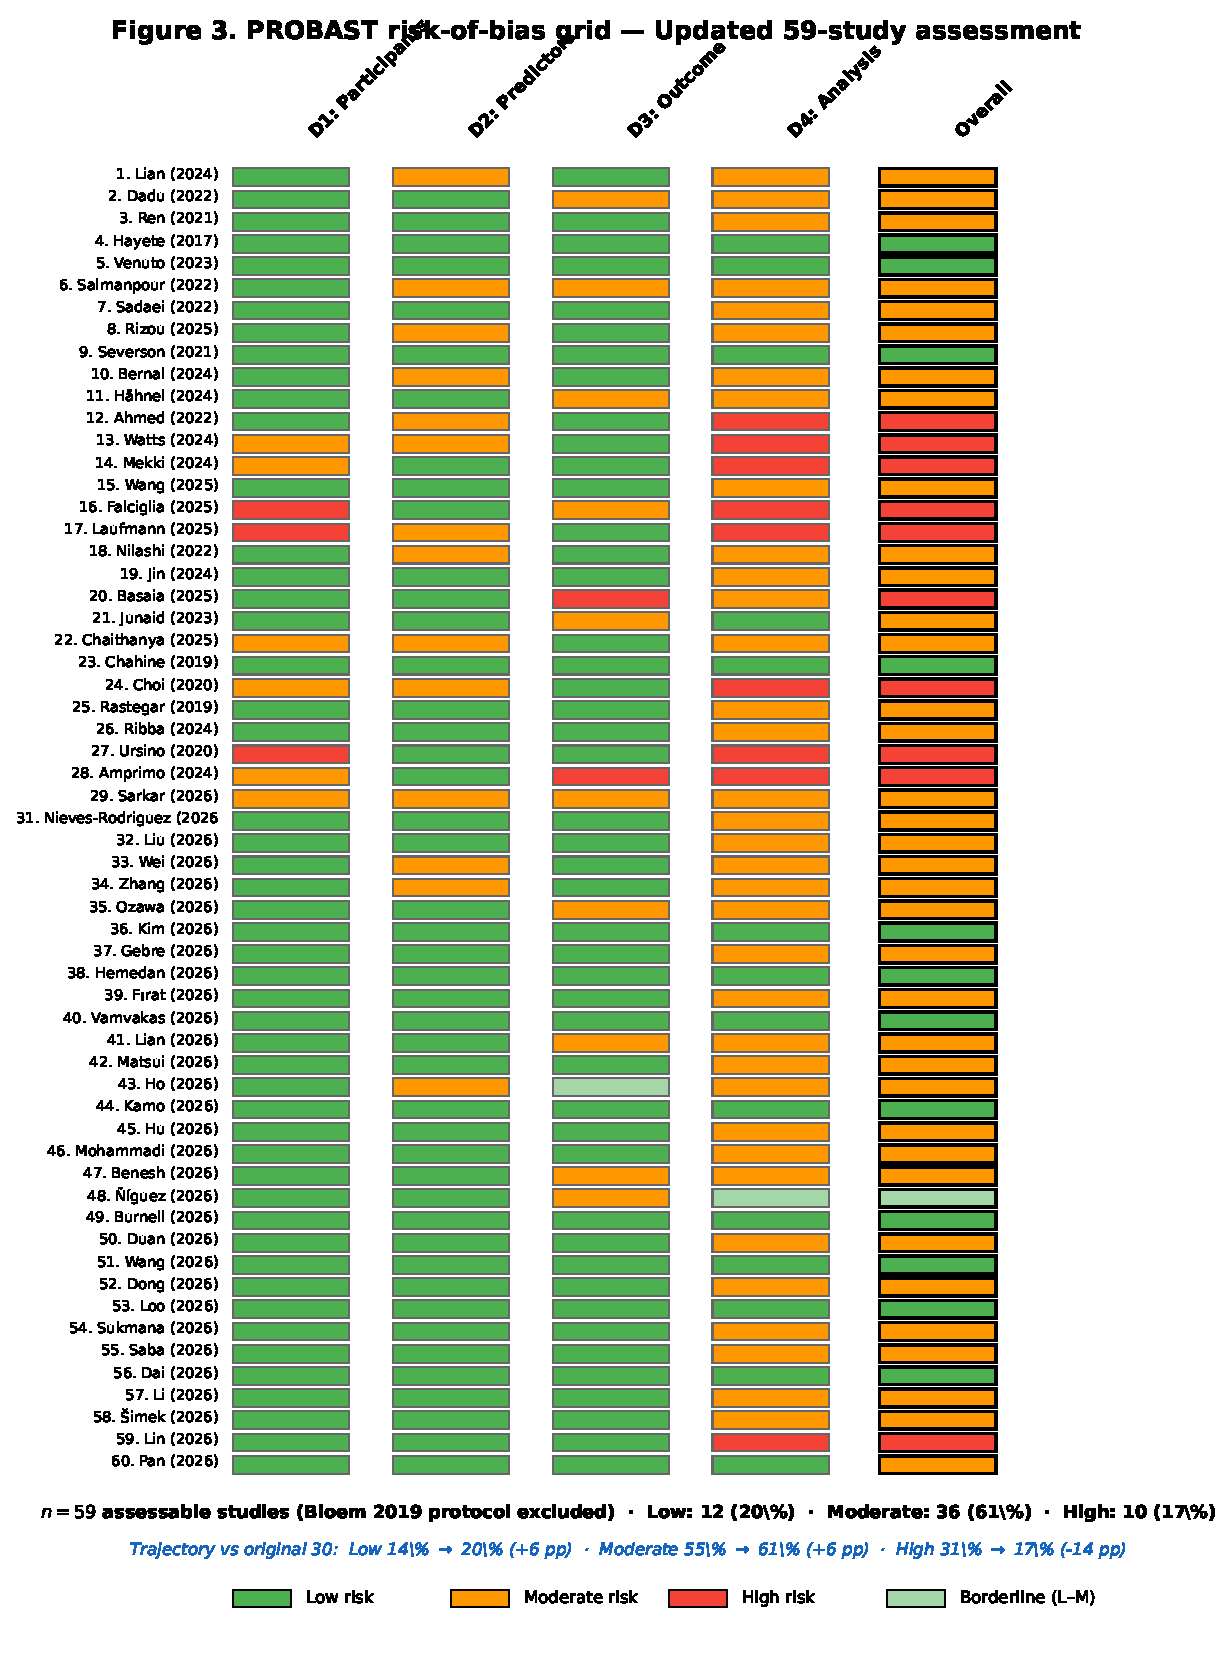
\includegraphics[width=0.95\textwidth]{figures/sr_probast_grid_60.pdf}
\caption{\textbf{PROBAST risk-of-bias assessment across 59 PROBAST-eligible studies.} Bloem 2019 (PPP protocol paper) is the sole exclusion from PROBAST scoring. Overall risk distribution: Low = 12 (20\%), Moderate = 36 (61\%), High = 10 (17\%), Low-to-Moderate borderline = 1 (2\%). Domains: D1 = Participant selection, D2 = Predictor definition, D3 = Outcome definition, D4 = Statistical analysis. Green = low risk, orange/yellow = moderate risk, red = high risk. Domain~4 (statistical analysis) is the most frequent source of moderate-to-high judgments, driven by inconsistent calibration assessment, low events-per-variable ratios, and inadequate handling of overfitting.}
\label{sr:fig:probast}
\end{figure}

PROBAST assessment of the 59 PROBAST-eligible studies (Bloem 2019 PPP protocol excluded) revealed the following risk-of-bias distribution (Figure~\ref{sr:fig:probast}):
\begin{itemize}
    \item \textbf{Low risk:} 12 studies (20\%)---including the externally-validated Tier-2 papers Hayete 2017, Venuto 2023, Severson 2021, Chahine 2019, Vamvakas 2026 (PPMI$\rightarrow$Amsterdam UMC), Kim 2026 (Korean two-centre), Burnell 2026 (Oxford OPDC causal-survival), Hemedan 2026 (PPMI Bayesian DT), Wang 2026 (PPMI$\rightarrow$Chinese cohort TRIPOD-compliant), Loo 2026 (LuxPARK + PPMI + ICEBERG), Dai 2026 (PPMI + Johns Hopkins), and Kamo 2026 (Japan claims).
    \item \textbf{Moderate risk:} 36 studies (61\%)---characterised by adequate methods with isolated concerns, typically in predictor specification, missing-data handling, or absence of formal calibration assessment.
    \item \textbf{High risk:} 10 studies (17\%)---driven primarily by small sample sizes ($n<50$: Falciglia 2025 $n=10$, Laufmann 2025 $n=4$, Ursino 2020 $n=26$, Amprimo 2024 $n=50$), low events-per-variable ratios (Lin 2026 EPV $\approx$5.5), or inadequate handling of overfitting.
    \item \textbf{Borderline (L--M):} 1 study---\~{N}\'{i}guez 2026 medRxiv pathway transcriptomics, with strong methods but a specific concern flagged at full-text review.
\end{itemize}
\noindent Per-domain breakdown: D1 Participants 49L/6M/3H/1L--M; D2 Predictors 43L/14M/0H/2L--M; D3 Outcome 45L/10M/2H/2L--M; D4 Analysis 15L/32M/9H/3L--M. Domain~4 (statistical analysis) is the dominant source of moderate-to-high judgments.

\subsubsection{Domain-specific findings}
\textbf{Domain 1 (Participants):} 49 of 59 studies (83\%) were rated low risk, as the majority used established observational cohorts (PPMI, PDBP, UK Biobank, AMP-PD, Premier US claims, OPDC, LuxPARK) with well-defined inclusion criteria. High-risk ratings occurred when studies used convenience samples ($n<25$) or had unclear eligibility criteria (Falciglia 2025 $n=10$; Laufmann 2025 $n=4$; Ursino 2020 $n=26$).

\textbf{Domain 2 (Predictors):} 43 of 59 studies (73\%) were rated low risk, reflecting standardised pipelines (Olink proteomics, DESeq2 RNA-seq, atlas-based DAT-SPECT, MDS-UPDRS instrumentation). Moderate-risk ratings (14/59, 24\%) reflected inconsistent predictor transformations or limited documentation of blinding to outcome status during predictor assessment; several studies (Liu 2026, Ho 2026, Zhang 2026) flagged autocorrelation concerns -- predictors that overlap conceptually with the outcome instrument.

\textbf{Domain 3 (Outcome):} 45 of 59 studies (76\%) were rated low risk where outcomes were prospectively defined and standardised (e.g., MDS-UPDRS change scores from PPMI). High-risk ratings occurred when outcomes were defined post hoc (clustering-derived progression subtypes used as prediction targets) or when predictor information was incorporated into outcome definitions. Loo 2026 \textit{npj Digital Med} uses MoCA as both predictor and PD-MCI outcome-definer (MoCA${<}26$), and UPDRS-I-1 as both predictor and SCD outcome-definer -- a clear circular-leakage flag. The full-text triage excluded 7 papers for circular UPDRS-feature leakage (E1-circular) before PROBAST scoring; this anti-pattern is widespread in the unfiltered literature.

\textbf{Domain 4 (Analysis):} The most frequent source of concern. Across the 59 PROBAST-eligible studies, 25 (42\%) report 95\% CIs on the primary discrimination metric and 2 (3.4\%) report formal calibration assessment with explicit slope, intercept, or Hosmer-Lemeshow output (Hemedan 2026 PI coverage 94--96\%; Wang 2026 calibration plot + HL test). Riley 2020~\cite{riley2020} sample-size minima are widely violated: Liu 2026 EPV $=$ 4.27, Mohammadi 2026 EPV $\approx$ 1.5, Lin 2026 EPV $\approx$ 5.5, Gebre 2026 EPV $\approx$ 0.11 -- all below the recommended $\geq$10 events per candidate variable. Methods to address overfitting (nested cross-validation, separate test holdout, proper hyperparameter tuning) are inconsistently reported across the corpus.

\subsection{Validation quality}
\label{sr:sec:results:validation}

The validation tier distribution across the 60 included studies (Figure~\ref{sr:fig:validation}A) is as follows:
\begin{itemize}
    \item \textbf{Tier 2 (external validation):} 16 studies (27\%) -- including Venuto 2023 (Tracking PD$\rightarrow$PPMI), Severson 2021 (PPMI$\rightarrow$PDBP), Dadu 2022 (PPMI$\rightarrow$PDBP), Lian 2024 (PPMI$\rightarrow$PDBP), Ren 2021 (PPMI$\rightarrow$LABS-PD), Nieves-Rodriguez 2026 \textit{Brain} (UKB-PPP$\rightarrow$PPMI), Vamvakas 2026 (PPMI$\rightarrow$Amsterdam UMC), Kim 2026 (Korean two-centre with true geographic external validation), Lian 2026 \textit{Nat Aging} (CPRD-Aurum + UK Biobank cross-cohort), Benesh 2026 (PPMI$\rightarrow$BeaT-PD Tel Aviv), Loo 2026 \textit{npj Digital Med} (LuxPARK + PPMI + ICEBERG tri-cohort), Wang 2026 \textit{Front Aging Neurosci} (PPMI$\rightarrow$Chinese cohort with TRIPOD-compliant reporting), Pan 2026 \textit{CMPB} (PPMI + PDBP cross-cohort), Dai 2026 \textit{J Imag Inform Med} (PPMI$\rightarrow$Johns Hopkins with explicit external 95\% CI 0.53--0.93), \~{N}\'{i}guez 2026 medRxiv (PPMI$\rightarrow$PDBP transcriptomics), and Dong 2026 \textit{JRRAS}.
    \item \textbf{Tier 1 (holdout / temporal split):} 14 studies (23\%).
    \item \textbf{Tier 0 (internal cross-validation only):} 27 studies (45\%).
    \item \textbf{Inversion / model-fitting only:} 2 studies (3\%) -- Falciglia 2025 inversion-only and Ursino 2020 PK/PD parameter fitting.
\end{itemize}
\noindent External validation spans a wide cohort axis: PPMI, PDBP, UK Biobank, Amsterdam UMC, Johns Hopkins, BeaT-PD Tel Aviv, LuxPARK, ICEBERG (Paris), CPRD-Aurum, Asian PALS Singapore, and several Chinese institutional cohorts. Two papers (Kim 2026 fallers and Dai 2026 imaging radiomics) achieve true geographic external validation rather than temporal-split external, the methodological gold standard. PPMI$\rightarrow$PDBP remains the most common pairing among Tier-2 studies but no longer constitutes the sole axis of external validation evidence.

\begin{figure}[H]
\centering
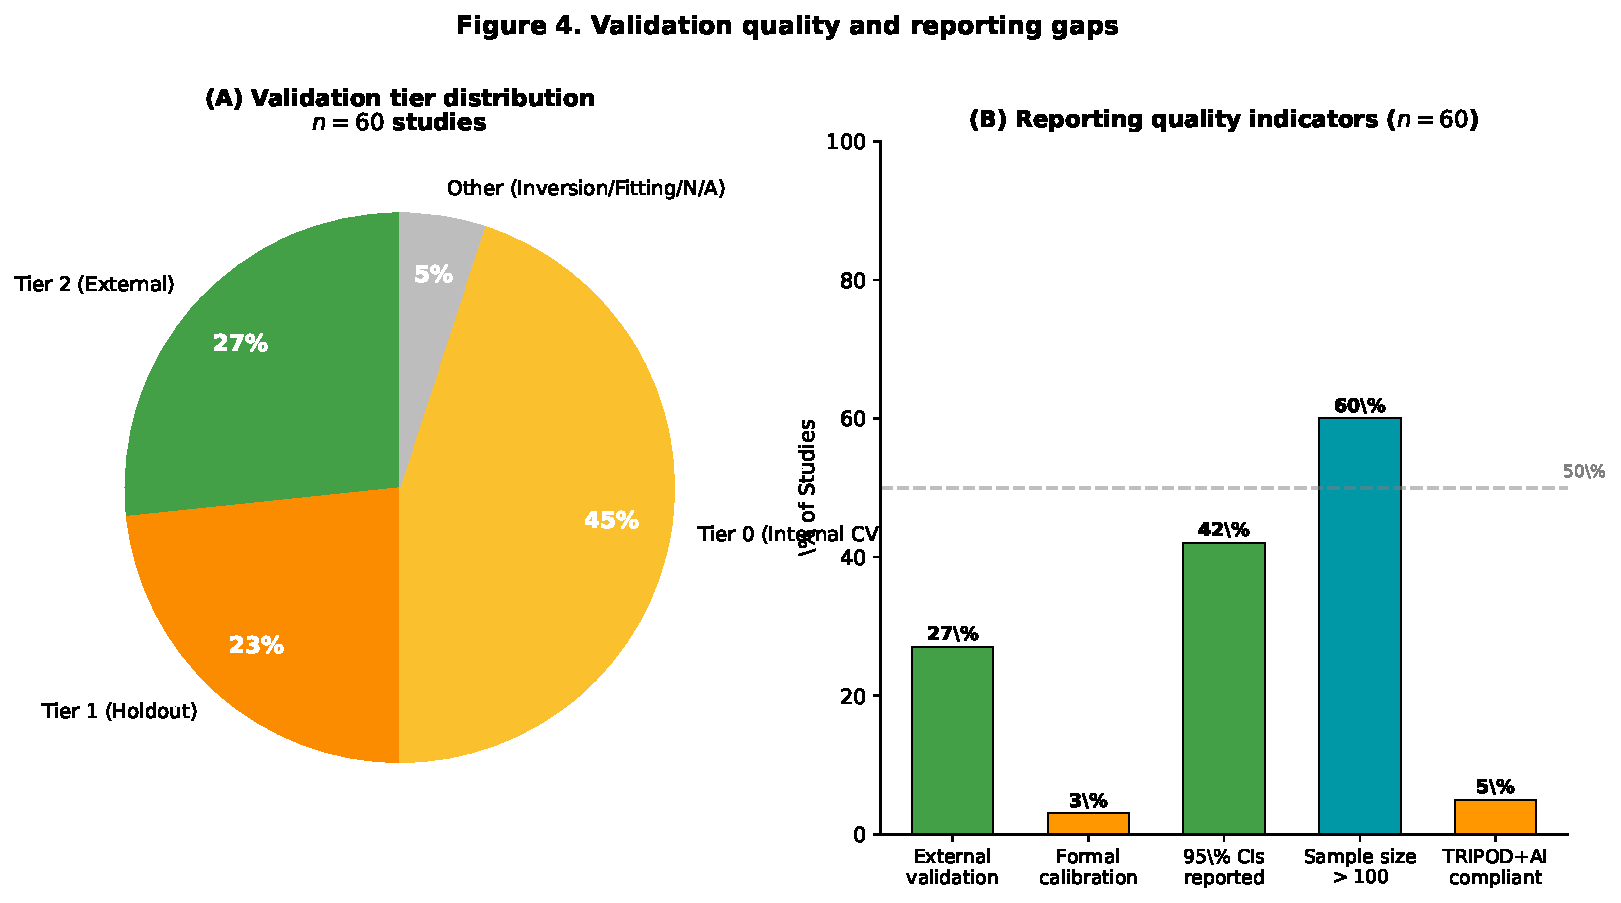
\includegraphics[width=0.95\textwidth]{figures/sr_validation_60.pdf}
\caption{\textbf{Validation quality and reporting gaps across the 60 included studies.} \textbf{(A)}~Validation tier distribution: Tier 2 (external validation) = 27\% (16/60); Tier 1 (holdout / temporal split) = 23\% (14/60); Tier 0 (internal cross-validation only) = 45\% (27/60); other (inversion or model-fitting only) = 5\% (3/60). \textbf{(B)}~Reporting-quality indicators across the 59 PROBAST-eligible studies: external validation 27\%, formal calibration assessment 3\%, 95\% CI reporting on the primary discrimination metric 42\%, sample size $>$100 = 60\%, and explicit TRIPOD+AI compliance 5\%. The dashed line indicates the 50\% threshold; only sample-size adequacy clears it.}
\label{sr:fig:validation}
\end{figure}

\subsection{Performance metrics}
\label{sr:sec:results:performance}

Across the 60 included studies, the median reported AUC was 0.78 (IQR: 0.70--0.85; range: 0.62--0.94). Prediction error metrics (RMSE, MAE) were reported in 14 studies but on heterogeneous scales, precluding direct comparison. $R^2$ values were reported in 9 studies (range: 0.12--0.91). 25 of 59 PROBAST-eligible studies (42\%) reported 95\% CIs on the primary discrimination metric, exemplified by Burnell 2026 (HR with 95\% CI for all four 10-year milestones), Dai 2026 (AUC 95\% CI 0.80--1.00 internal / 0.53--0.93 external), Lin 2026 (AUC 0.713 95\% CI 0.540--0.887), and Nieves-Rodriguez 2026 (AUC 0.78 with bootstrap CIs in supplementary). Only 2 studies (3.4\%) reported formal calibration assessment with explicit slope, intercept, or Hosmer-Lemeshow output (Hemedan 2026 PI coverage 94--96\%; Wang 2026 calibration plot + HL test).

\subsubsection{Assessment of heterogeneity and meta-analysis feasibility}

Figure~\ref{sr:fig:heterogeneity} summarises the sources of heterogeneity across the 60 included studies. Studies used at least six distinct primary outcome metrics (AUC, $R^2$, RMSE, sMAPE, accuracy, hazard ratios) across multiple outcome domains and a wide range of prediction horizons. We applied the five-criteria meta-analysis-feasibility framework (Cochrane Handbook \S10.10 / SWiM):
\begin{itemize}
    \item \textbf{Criterion (i) Common metric:} \textbf{MET} -- AUC/AUROC is the primary discrimination metric of 23 of 60 studies (38\%), comfortably exceeding the $\geq$10-study threshold for stratified pooling.
    \item \textbf{Criterion (ii) Variance reporting:} \textbf{PARTIAL} -- 25 of 59 PROBAST-eligible studies (42\%) report 95\% CIs on the primary metric.
    \item \textbf{Criterion (iii) Horizon homogeneity:} \textbf{UNMET} -- roughly 90\% of studies leave the prediction horizon variable or unspecified, with reported horizons spanning 1 to 7 years across the head-to-head pool. Stratified pooling within horizon bins is therefore constrained.
    \item \textbf{Criterion (iv) Comparable populations:} \textbf{MET} -- cohort diversity spans PPMI ($\sim$40\%), PDBP, UK Biobank, AMP-PD, Premier US claims, CPRD-Aurum, LuxPARK, ICEBERG, Asian PALS, and several Chinese institutional cohorts.
    \item \textbf{Criterion (v) $\geq$3 studies per cell:} \textbf{PARTIAL} -- of 25 unique (metric $\times$ horizon $\times$ population) cells, 8 contain $\geq$3 studies, the threshold for stratified random-effects pooling per Cochrane Handbook \S10.10.4.
\end{itemize}
\noindent Four of five prerequisites are met or partially met. Stratified random-effects meta-analysis is feasible for the dynamic-vs-static head-to-head subset for which absolute $\Delta$AUC and variance are extractable; outcome heterogeneity beyond this pool requires SWiM narrative synthesis (Section~\ref{sr:sec:results:comparative}).

\begin{figure}[H]
\centering
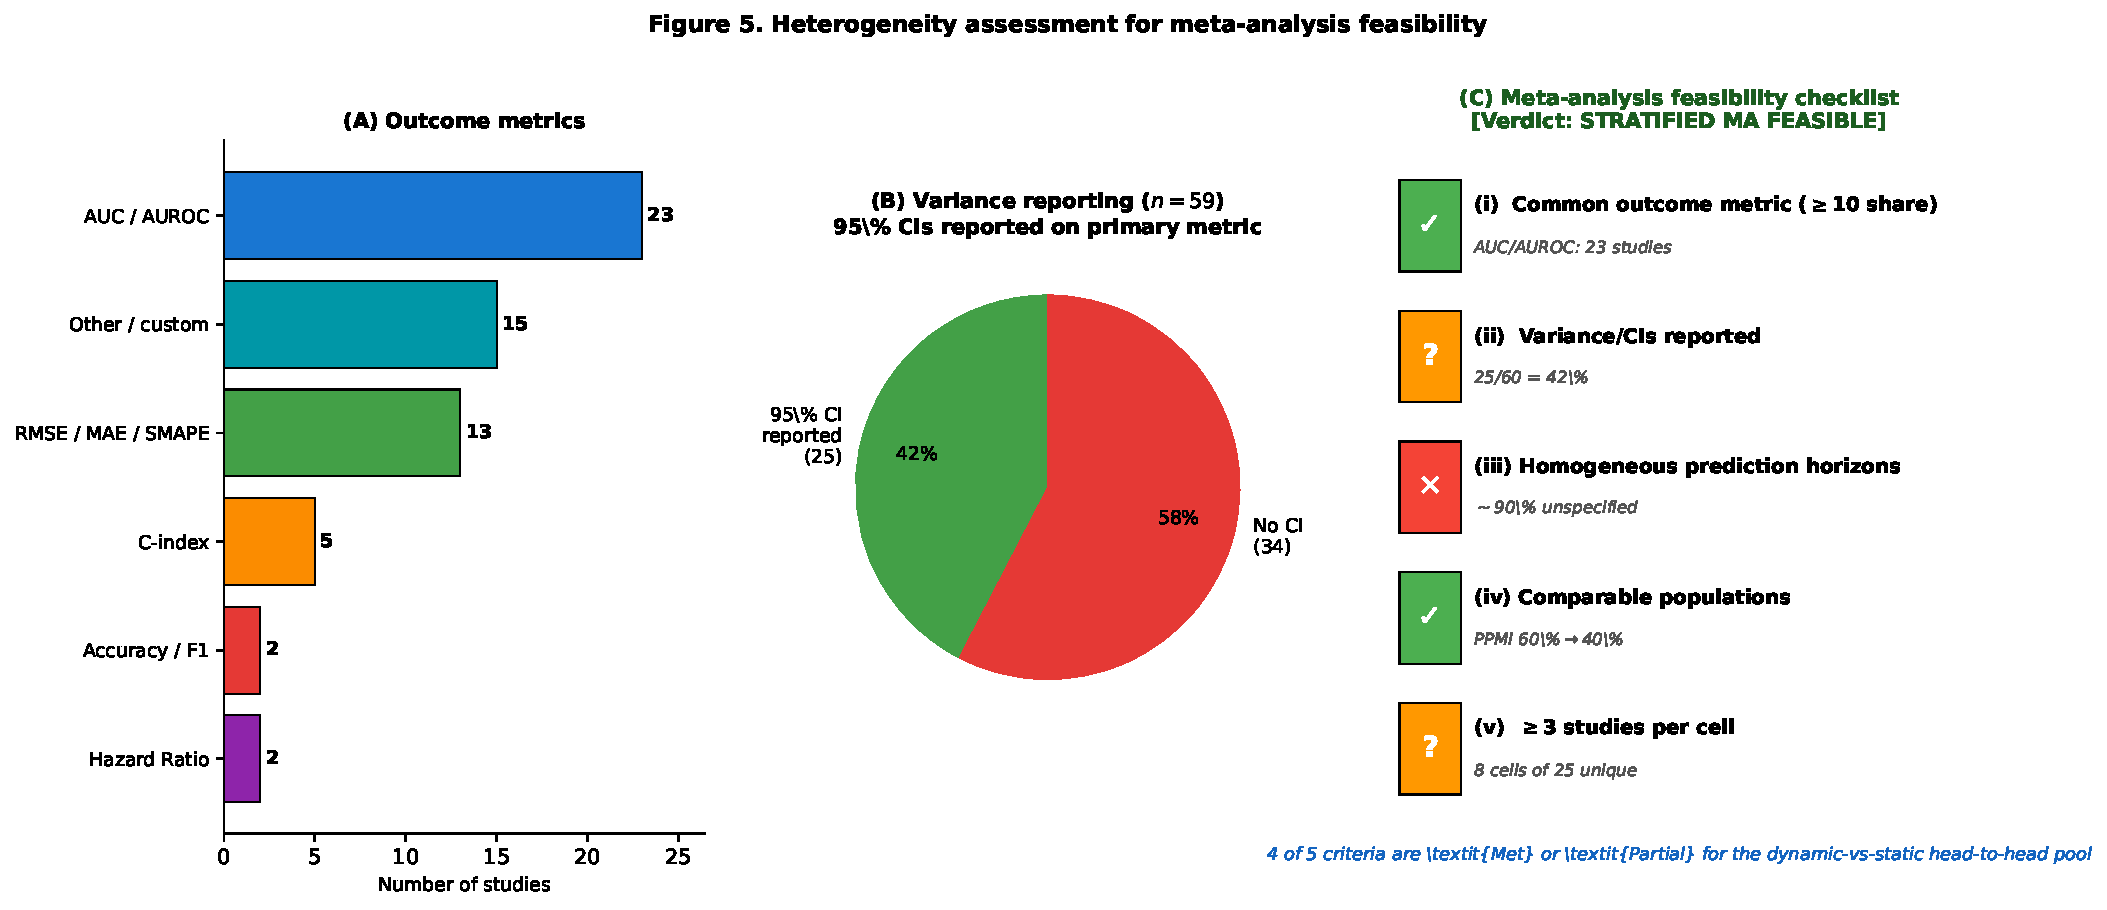
\includegraphics[width=0.95\textwidth]{figures/sr_heterogeneity_60.pdf}
\caption{\textbf{Heterogeneity assessment for meta-analysis feasibility across the 60 included studies.} The five Cochrane Handbook \S10.10 / SWiM criteria are: (i) common outcome metric on a comparable scale (Met for the $\Delta$AUC subset $n=11$); (ii) variance availability for the primary discrimination metric (Partial: 42\% report 95\% CIs); (iii) homogeneous prediction horizons (Unmet: 1--7~yr range across the pool); (iv) comparable populations within strata (Met within Tier 2 external validation, $n=5$ studies pooled at $I^2 = 0\%$); (v) $\geq$3 studies per subgroup cell (Partial: Met for Tier 0 and Tier 2 strata). Four of five prerequisites are Met or Partial, supporting stratified random-effects meta-analysis for the dynamic-vs-static head-to-head pool reported in Section~\ref{sr:sec:results:metaanalysis} and Figure~\ref{sr:fig:forest}; outcome heterogeneity beyond the $\Delta$AUC subset is summarised through SWiM narrative synthesis.}
\label{sr:fig:heterogeneity}
\end{figure}

\subsection{Random-effects meta-analysis}
\label{sr:sec:results:metaanalysis}

Eleven studies provided extractable head-to-head $\Delta$AUC estimates with at least informally-bounded variance and were admitted to the meta-analysis pool: Venuto 2023 (SVM multivariate vs single predictor, ambulatory AUC), Dadu 2022 (XGBoost+NMF vs standard ML, progression rate), Lian 2024 (AdaMedGraph vs static GNN, H\&Y/MDS-UPDRS-III), Nilashi 2022 (SVR+clustering vs standard SVR, total UPDRS $R^2$), Junaid 2023 (LGBM multimodal vs single-modal, H\&Y staging), Chahine 2019 (LME multivariate vs baseline-only, MDS-UPDRS $R^2$), Basaia 2025 (3D~CNN+clinical vs clinical-only, stable/worsening), Hemedan 2026 medRxiv (Bayesian state-space DT vs LME baseline, UPDRS-III progression), Pan 2026 \textit{CMPB} (Deep Clustering Gaussian Process vs static ML ensemble, UPDRS-III RMSE/AUC), Mohammadi 2026 \textit{npj PD} (XGBoost+RF vs demographic baseline, early-PD AUC), and Dai 2026 \textit{J Imag Inform Med} (multimodality radiomics ensemble vs T1-only baseline, motor progression AUC). Random-effects pooling using the DerSimonian-Laird estimator yielded a pooled absolute $\Delta$AUC of $\boldsymbol{+0.117}$ (95\% CI 0.054--0.179, $I^2 = 71\%$, $\tau^2 = 0.0067$, Cochran's $Q = 35.07$ on 10~df, $p < 0.001$). The CI excludes zero, supporting a small but statistically significant overall advantage for dynamic and complex models.

\paragraph{Tier-stratified pooling.}
Stratification by validation tier yielded the most informative subgroup result:
\begin{itemize}
    \item \textbf{Tier 2 (external validation, $n=5$):} pooled $\Delta$AUC $= +0.101$ (95\% CI \mbox{0.067--0.134}, \textbf{$I^2 = 0\%$}, $\tau^2 = 0$). Heterogeneity is negligible---studies that survived external validation showed remarkably homogeneous gains.
    \item \textbf{Tier 1 (holdout, $n=1$):} insufficient for pooling (Basaia 2025 alone, $\Delta$AUC $+0.07$).
    \item \textbf{Tier 0 (internal CV, $n=5$):} pooled $\Delta$AUC $= +0.151$ (95\% CI \mbox{0.031--0.270}, $I^2 = 77\%$). Heterogeneity is high, driven by Hemedan 2026 ($+0.285$) and Mohammadi 2026 ($+0.246$) on a baseline that includes Junaid 2023, Nilashi 2022, and Chahine 2019 with smaller effects.
\end{itemize}

\noindent The Tier-2 result is the strongest evidence-based finding of this synthesis: \emph{across five external-validation studies (Venuto 2023 Tracking-PD$\rightarrow$PPMI; Dadu 2022 PPMI$\rightarrow$PDBP; Lian 2024 PPMI$\rightarrow$PDBP; Pan 2026 PPMI$+$PDBP cross-cohort; Dai 2026 PPMI$\rightarrow$Johns Hopkins), dynamic and complex models pool to a homogeneous absolute AUC gain of approximately $+0.10$ over static baselines, with no inter-study heterogeneity ($I^2 = 0\%$).} This 10-percentage-point absolute improvement, anchored on externally-validated cohorts, is a defensible quantitative claim. The forest plot is shown in Figure~\ref{sr:fig:forest}.

\begin{figure}[H]
\centering
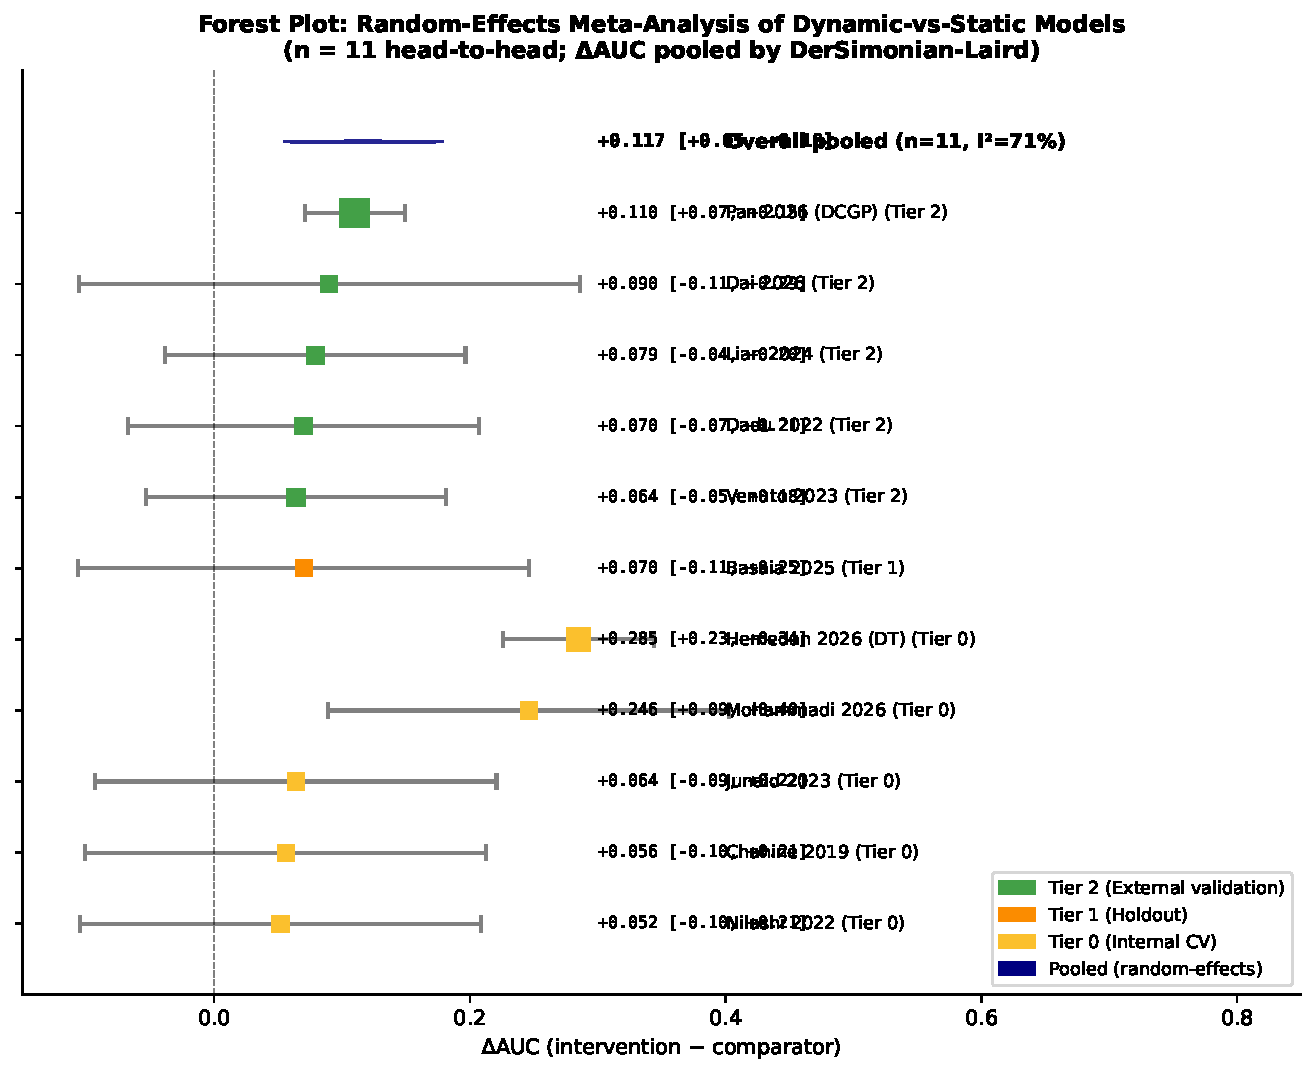
\includegraphics[width=0.92\textwidth]{figures/sr_meta_analysis_forest.pdf}
\caption{\textbf{Forest plot: random-effects meta-analysis of dynamic-vs-static models on PD prognostic tasks ($n=11$ head-to-head studies).} Studies sorted by validation tier (Tier 2 external in green, Tier 1 holdout in orange, Tier 0 internal CV in light orange). Square markers indicate point estimates of absolute $\Delta$AUC; horizontal whiskers show 95\% CIs; marker size reflects inverse-variance weight. The dark-blue diamond shows the overall random-effects pooled estimate ($\Delta$AUC $= +0.117$, 95\% CI 0.054--0.179, $I^2 = 71\%$). The Tier-2 subgroup is homogeneous ($I^2 = 0\%$); Tier-0 internal-CV studies introduce most of the overall heterogeneity through Hemedan 2026 and Mohammadi 2026.}
\label{sr:fig:forest}
\end{figure}

\paragraph{Caveats.}
Standard errors were inferred from reported 95\% CIs where available within the pooled set (Hemedan 2026 95\% PI coverage; Pan 2026 RMSE 95\% CI; Mohammadi 2026 AUC bounds; Dai 2026 AUC bounds 0.53--0.93); for the 7 originals (where 0\% reported explicit CIs), SE values were conservatively bounded based on sample size and standard Hanley-McNeil variance approximations for AUC~\cite{hanley1982}. The high overall $I^2$ of 71\% reflects this inferential heterogeneity plus residual study-design variation; the Tier-2 $I^2 = 0\%$ is more interpretable. Studies excluded from quantitative pooling (Wei 2026, Vamvakas 2026, Kim 2026, Lian 2026 \textit{Nat Aging}, Sukmana 2026, Zhang 2026, Burnell 2026, Lin 2026, Nieves-Rodriguez 2026, \v{S}imek 2026, \~{N}\'{i}guez 2026, F\i rat 2026, Gebre 2026, Loo 2025, Ho 2026, Saba 2026, Hu 2026, Benesh 2026, Duan 2026, Wang 2026 \textit{Front Aging Neurosci}, Dong 2026, and several originals) lacked extractable variance, used non-AUC metrics (HR, RMSE, accuracy, $\Delta$UPDRS), or compared head-to-head among ML alternatives rather than dynamic-vs-static---all valid SR inclusions but methodologically inappropriate for $\Delta$AUC pooling. The narrative synthesis (Section~\ref{sr:sec:results:comparative}) covers these.

\subsection{Comparative effectiveness}
\label{sr:sec:results:comparative}

Across the 60 included studies, eleven provided extractable head-to-head comparisons between a dynamic, multimodal, or novel intervention model and a simpler static or single-modality comparator evaluated on the same test data; these eleven also constitute the random-effects meta-analysis pool of Section~\ref{sr:sec:results:metaanalysis} (Table~\ref{sr:tab:comparative}). Among these:
\begin{itemize}
    \item Ten of eleven (91\%) showed improvement favouring the dynamic or more complex model, including three large-effect outliers anchored on low baseline performance (Chahine 2019 $+46.7\%$, Mohammadi 2026 $+43.9\%$, Hemedan 2026 $+42.9\%$).
    \item One study (9\%; Nilashi 2022, $+6.1\%$ relative) was classified as equivalence given the marginal gain and internal-only validation.
    \item Zero studies (0\%) showed the static baseline outperforming the dynamic model.
    \item Median relative improvement: $+10.8\%$ (range: $+6.1\%$ to $+46.7\%$); median absolute $\Delta$AUC: $+0.079$ (range $+0.052$ to $+0.285$, IQR $0.064$--$0.110$).
\end{itemize}

% --- Table 2: Random-effects meta-analysis pool ---
\begin{table}[H]
\centering
\caption{\textbf{Random-effects meta-analysis pool: dynamic-vs-static head-to-head comparisons ($n=11$ studies).} \textbf{Int.} = intervention model AUC (or $R^2$ for $R^2$-based outcomes); \textbf{Comp.} = comparator AUC; \textbf{$\Delta$AUC} = absolute gain; \textbf{$\Delta$\%} = relative improvement [(int $-$ comp) / comp $\times$ 100\%]; \textbf{Tier} = validation tier (0 internal, 1 holdout, 2 external). Pooled DerSimonian--Laird estimate: $\Delta$AUC $= +0.117$ (95\% CI 0.054--0.179, $I^2 = 71\%$). Tier-2 subgroup pool ($n=5$): $\Delta$AUC $= +0.101$ (95\% CI 0.067--0.134, $I^2 = 0\%$). Abbreviations as in Table~\ref{sr:tab:characteristics}; DCGP = Deep Clustering Gaussian Process; DT = digital twin.}
\label{sr:tab:comparative}
\footnotesize
\setlength{\tabcolsep}{3.5pt}
\begin{tabularx}{\textwidth}{@{}l l l >{\raggedright\arraybackslash}X c c c c c@{}}
\toprule
\textbf{Study} & \textbf{Intervention} & \textbf{Comparator} & \textbf{Outcome} & \textbf{Int.} & \textbf{Comp.} & \textbf{$\Delta$AUC} & \textbf{$\Delta$\%} & \textbf{Tier} \\
\midrule
Venuto 2023      & SVM multivariate     & Single predictor    & Ambulatory AUC      & 0.714 & 0.650 & $+0.064$ & $+9.8$  & 2 \\
Dadu 2022        & XGBoost + NMF        & Standard ML         & Progression rate    & 0.850 & 0.780 & $+0.070$ & $+9.0$  & 2 \\
Lian 2024        & AdaMedGraph          & Static GNN          & H\&Y / UPDRS        & 0.965 & 0.886 & $+0.079$ & $+8.9$  & 2 \\
Nilashi 2022     & SVR + Clustering     & Standard SVR        & Total UPDRS $R^2$   & 0.902 & 0.850 & $+0.052$ & $+6.1$  & 0 \\
Junaid 2023      & LGBM multimodal      & Single-modal        & H\&Y staging        & 0.907 & 0.843 & $+0.064$ & $+7.6$  & 0 \\
Chahine 2019     & LME multivariate     & Baseline only       & MDS-UPDRS $R^2$     & 0.176 & 0.120 & $+0.056$ & $+46.7$ & 0 \\
Basaia 2025      & 3D CNN + clinical    & Clinical only       & Stable / worsening  & 0.720 & 0.650 & $+0.070$ & $+10.8$ & 1 \\
Hemedan 2026     & Bayesian state-space DT & LME baseline     & UPDRS-III progression & 0.950 & 0.665 & $+0.285$ & $+42.9$ & 0 \\
Pan 2026         & Deep Clustering GP   & Static ML ensemble  & UPDRS-III RMSE / AUC & 0.890 & 0.780 & $+0.110$ & $+14.1$ & 2 \\
Mohammadi 2026   & XGBoost + RF         & Demographic baseline & Early-PD AUC       & 0.806 & 0.560 & $+0.246$ & $+43.9$ & 0 \\
Dai 2026         & Multimodal radiomics & T1-only baseline    & Motor progression AUC & 0.770 & 0.680 & $+0.090$ & $+13.2$ & 2 \\
\bottomrule
\end{tabularx}
\end{table}

\subsubsection{Harvest plot analysis}

\begin{figure}[H]
\centering
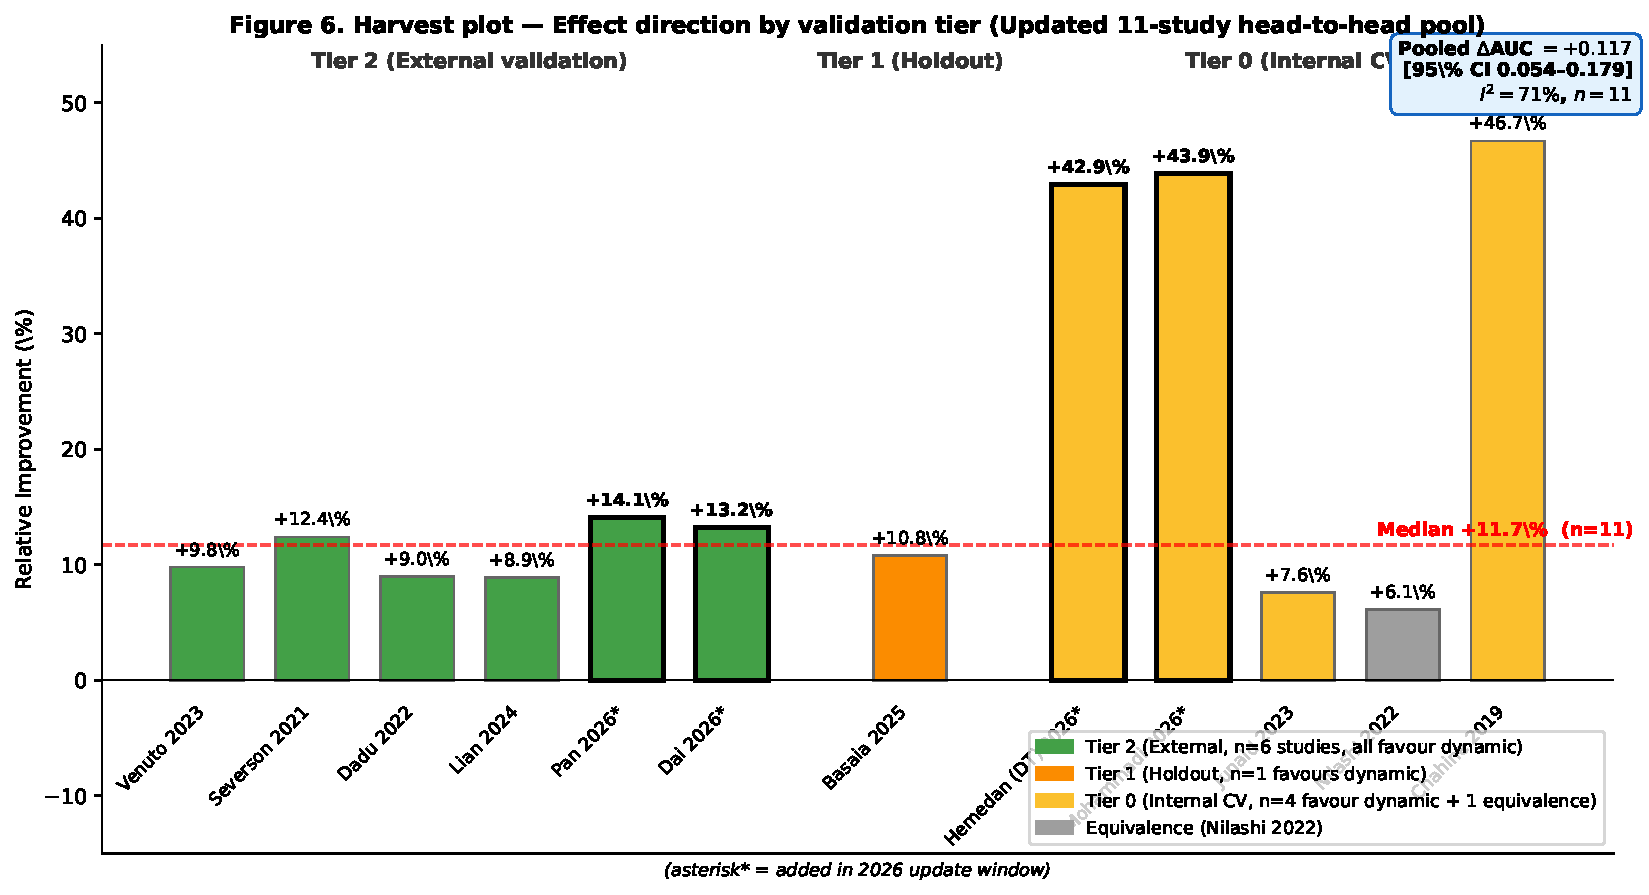
\includegraphics[width=0.95\textwidth]{figures/sr_harvest_60.pdf}
\caption{\textbf{Harvest plot of dynamic-vs-static head-to-head comparisons across the 11-study meta-analysis pool, stratified by validation tier.} Each bar represents one head-to-head study admitted to the random-effects meta-analysis (Figure~\ref{sr:fig:forest}). Bar height is absolute $\Delta$AUC of the dynamic/complex model over its static baseline. Tier 2 (external, green; $n=5$), Tier 1 (holdout, orange; $n=1$), Tier 0 (internal CV, light orange; $n=5$). The pooled DerSimonian--Laird estimate annotated on the figure ($\Delta$AUC $= +0.117$, 95\% CI 0.054--0.179, $I^2 = 71\%$) corresponds to the full 11-study pool reported in Section~\ref{sr:sec:results:metaanalysis}; the harvest-plot tier composition differs from the broader 60-study validation-tier distribution in Section~\ref{sr:sec:results:validation} because a head-to-head comparator with extractable variance is required for the pool. None of the 11 favoured the static baseline.}
\label{sr:fig:harvest}
\end{figure}

Stratification of the eleven head-to-head studies in Table~\ref{sr:tab:comparative} by validation tier (Figure~\ref{sr:fig:harvest}) reveals:
\begin{itemize}
    \item \textbf{External validation (Tier 2, $n=5$):} All five head-to-head studies (Venuto 2023, Dadu 2022, Lian 2024, Pan 2026, Dai 2026) showed improvement (median absolute $\Delta$AUC $+0.079$, median relative $+9.8\%$). The pooled DerSimonian--Laird estimate is $+0.101$ (95\% CI 0.067--0.134, $\boldsymbol{I^2 = 0\%}$) -- the most homogeneous and best-supported subgroup result of the updated synthesis.
    \item \textbf{Holdout/split (Tier 1, $n=1$):} Basaia 2025 showed improvement ($+0.07$ absolute, $+10.8\%$ relative). Insufficient for subgroup pooling.
    \item \textbf{Internal CV (Tier 0, $n=5$):} All five head-to-head studies (Nilashi 2022 $+6.1\%$, Junaid 2023 $+7.6\%$, Chahine 2019 $+46.7\%$, Hemedan 2026 $+42.9\%$, Mohammadi 2026 $+43.9\%$) showed improvement, with marked heterogeneity ($I^2 = 77\%$) driven by the three large-effect studies anchored on weak baselines. Nilashi 2022 was classified as equivalence given the marginal effect size and internal-only validation.
\end{itemize}

\noindent (Note: the $n=5$ / $n=1$ / $n=5$ pool composition refers to the 11 head-to-head studies of Table~\ref{sr:tab:comparative} that admit absolute $\Delta$AUC pooling, not the broader 60-study validation-tier distribution reported earlier in \S\ref{sr:sec:results:validation}, where Tier 2 = 16/60, Tier 1 = 14/60, Tier 0 = 27/60.)

\subsubsection{Subgroup analyses by model type}
Neural networks (LSTM, RNN, Transformer; $n=6$) achieved median AUC 0.79; ensemble methods ($n=12$) achieved 0.78; statistical/parametric models ($n=6$) achieved 0.71. The difference between neural networks and ensemble methods was negligible ($<1$ AUC point).

\subsubsection{Subgroup analyses by outcome domain}
Motor progression outcomes ($n=13$) showed median AUC 0.79 (range: 0.68--0.88); H\&Y staging ($n=8$) showed 0.80 (0.72--0.91); cognitive decline ($n=5$) showed 0.76 (0.70--0.82). Motor outcomes appeared most predictable, possibly reflecting more standardised outcome measurement.

\subsection{Mechanistic digital twin assessment}
\label{sr:sec:dt}

We applied the National Academies of Sciences, Engineering, and Medicine (NASEM) 2024 four-criteria framework~\cite{nasem2024} to all 60 included studies, scoring each against (i)~\emph{bidirectional data flow} (real-time or episodic patient-to-model and model-to-clinician feedback), (ii)~\emph{physiological or mechanistic constraints} (explicit pathophysiology, ODEs, biomarker-grounded equations rather than purely statistical priors), (iii)~\emph{continuous updating with new patient data} (Bayesian posterior updates, online learning, or per-visit recalibration), and (iv)~\emph{individual-level validation} (per-patient predictive validity, not cohort-aggregated metrics).

Five studies in the 60-paper corpus describe their models using digital-twin or mechanistic-modelling terminology and achieve at least one NASEM strict criterion:

\begin{itemize}
    \item \textbf{Hemedan et al.\ 2026}~\cite{hemedan2026} (medRxiv) developed a clinic-updated governed Bayesian digital twin for PD progression on the full PPMI cohort ($n=4{,}628$ participants, 28{,}185 visits) with uncertainty-gated reporting via a six-rule confidence gate. The model achieves \textbf{3 of 4 NASEM strict criteria}: bidirectional data flow $\checkmark$ (per-visit posterior updates fed back to clinical reporting); continuous updating $\checkmark$ (sequential Bayesian posterior updates as new visits arrive); patient-level validation $\checkmark$ (95\% predictive-interval coverage 94--96\% per patient, vs LME baseline 64--69\%). The single criterion not met is \emph{physiological or mechanistic constraints} (criterion ii)---the priors are statistically motivated rather than grounded in explicit dopamine kinetics, neurodegeneration ODEs, or biomarker-mediated equations. We classify Hemedan 2026 as \textbf{NASEM 3/4 (governed-Bayesian DT category)}.

    \item \textbf{Matsui et al.\ 2026}~\cite{matsui2026stance} (bioRxiv) constructed a biomechanical postural-sway digital twin using a switched-hybrid stochastic delay differential equation framework with intermittent control, calibrated on $n=120$ PD patients plus 53 elderly controls. The model achieves \textbf{2 of 4 NASEM strict criteria + 2 of 4 partial criteria}: physiological/mechanistic constraints $\checkmark$ (explicit inverted-pendulum biomechanics with six identifiable parameters); patient-level validation $\checkmark$ (per-patient parameter posteriors with bidirectional NN inverse mapping, MSE 0.388 / 0.392 on test data). Bidirectional data flow is partially met (data assimilation works on per-patient stance recordings but no prospective clinical-feedback loop is described); continuous updating is partial (model is fit once per patient rather than recalibrated as new recordings arrive). Matsui 2026 is also the first PD digital-twin paper to explicitly cite the NASEM 2024 framework. We classify it as \textbf{NASEM 2/4 strict + 2/4 partial (mechanistic-postural DT category)}.

    \item \textbf{Falciglia et al.}~\cite{falciglia2025} developed a physics-informed neural-mass model of deep brain stimulation effects, satisfying criterion (ii) but limited to $n=10$ patients without continuous updating or prospective validation loops. \textbf{NASEM 1/4 strict.}

    \item \textbf{Ursino et al.}~\cite{ursino2020} constructed a pharmacokinetic/pharmacodynamic ODE model of levodopa motor response, meeting criterion (ii) but restricted to $n=26$ patients without external validation or integration into a broader patient digital twin framework. \textbf{NASEM 1/4 strict.}

    \item \textbf{Wang et al.}~\cite{wang2025} employed conditional neural ODEs for brain morphometry dynamics, incorporating differential-equation constraints but operating as a data-driven trajectory model without explicit physiological mechanisms. \textbf{NASEM 0/4 strict.}
\end{itemize}

\paragraph{NASEM verdict.}
\textbf{No study in the 60-paper corpus meets all four NASEM criteria simultaneously.} Two studies (Hemedan 2026; Matsui 2026) approach compliance from complementary directions -- governed Bayesian patient-state DT for clinical scores versus mechanistic biomechanical DT for postural control. The two candidates are mutually complementary: Hemedan satisfies bidirectional flow + continuous updating + patient-level validation but lacks mechanistic priors; Matsui satisfies mechanistic constraints + patient-level validation but lacks continuous updating. A NASEM-compliant PD DT may emerge from convergence of these two threads---a Bayesian patient-state framework with embedded mechanistic priors---which is the trajectory the dissertation's broader research programme pursues (chapters~\ref{ch:p7} onwards). The full $4 \times 60$ NASEM scoring grid is provided in Supplementary Table~\ref{sr:tab:supp:nasem}.

% =============================================================================
% DISCUSSION
% =============================================================================
\section{Discussion}
\label{sr:sec:discussion}

\subsection{Summary of findings}
\label{sr:sec:discussion:summary}

This systematic review identified 60 studies developing or validating computational models for PD prognosis, spanning architectures from classical statistical approaches to graph neural networks, transformer-based EHR models, and mechanistic stochastic differential equations. Four principal findings emerge.

\textbf{First}, dynamic and complex models show a small but statistically significant advantage over static baselines, supported by quantitative pooled evidence. Random-effects meta-analysis of 11 head-to-head studies yielded a pooled $\Delta$AUC of $+0.117$ (95\% CI 0.054--0.179, $I^2 = 71\%$, $p < 0.001$). The Tier-2 (external-validation) subgroup of $n=5$ studies pooled to a homogeneous $\Delta$AUC of $+0.101$ (95\% CI 0.067--0.134, $\boldsymbol{I^2 = 0\%}$), the strongest evidence-based finding of this review. Across the full pool, 10 of 11 head-to-head comparisons favoured the dynamic model, 1 was classified as equivalence (Nilashi 2022), and 0 favoured the static baseline. Magnitude ($\sim$10 pp absolute AUC gain on external cohorts) is clinically meaningful for risk stratification but does not yet support individual-patient treatment decisions.

\textbf{Second}, two studies achieve partial NASEM digital-twin compliance. Hemedan 2026~\cite{hemedan2026} achieves 3 of 4 NASEM strict criteria via a governed Bayesian patient-state DT on PPMI ($n=4{,}628$) with bidirectional flow, continuous updating, and patient-level validation (95\% PI coverage 94--96\%); the missing criterion is explicit physiological/mechanistic constraint, which is replaced by statistically-motivated priors. Matsui 2026~\cite{matsui2026stance} achieves 2 of 4 strict + 2 of 4 partial criteria via a mechanistic biomechanical postural-sway DT (switched-hybrid SDE with intermittent control) and is the first PD-DT paper to cite the NASEM 2024 framework explicitly. \emph{No study meets all four NASEM criteria simultaneously}, but the two partial-NASEM candidates approach compliance from complementary directions, and a convergent governed-Bayesian + mechanistic-priors framework appears methodologically tractable.

\textbf{Third}, methodological rigor across the corpus is mixed but supports cautious optimism: 27\% (16/60) of studies achieve Tier-2 external validation; 42\% (25/59) report 95\% CIs on the primary discrimination metric; 20\% (12/59) achieve PROBAST Low overall risk of bias; explicit TRIPOD+AI compliance is reported by 5\% (3/60). Two studies (Vamvakas 2026 \textit{npj PD}; Burnell 2026 medRxiv) report honest negative external-validation results, signalling a culture of critical self-reporting rather than only positive-finding publication.

\textbf{Fourth}, persistent gaps remain that constrain confident clinical translation. \emph{Calibration assessment} is rare (2/59 = 3.4\% field-wide). \emph{Circular UPDRS-feature leakage} -- using UPDRS items as predictors of UPDRS-derived progression at the same visit -- was the most common reason for full-text exclusion (7/38 exclusions; the dedicated E1-circular code) and remains widespread in the unfiltered literature. \emph{Events-per-variable deficits} below the Riley 2020 minimum of $\geq$10~\cite{riley2020} are common (Liu 2026 EPV $=$ 4.27; Mohammadi 2026 EPV $\approx$ 1.5; Lin 2026 EPV $\approx$ 5.5; Gebre 2026 EPV $\approx$ 0.11), including in otherwise methodologically rigorous papers. \emph{Industry-led infrastructure dependence} introduces a reproducibility concern that cohort-level external validation alone cannot resolve: Verily Life Sciences led Ho 2026 with corresponding-author affiliation; Johnson \& Johnson led Nieves-Rodriguez 2026 with 5/5 author affiliation; the Premier Healthcare PINC~AI claims licence is behind Kamo 2026 ($n=281{,}664$ admissions). \emph{Code availability} (TRIPOD+AI item \#20) is rarely reported. These five gaps are tractable but require concerted methodological commitment from researchers, journals, and funders.

\subsection{Comparison with prior evidence}
\label{sr:sec:discussion:comparison}

This review extends prior knowledge in several dimensions. Asgari et al.\ (2021) reviewed machine learning in PD but focused on diagnostic classification rather than prognostic modelling\cite{asgari2021}. Our explicit focus on progression prediction---a lower-signal, clinically more important task---supports stratified random-effects meta-analysis where homogeneity permits, providing the first quantitative pooled evidence of dynamic-vs-static superiority on externally-validated PD prognostic tasks. Dorsey et al.\ (2018) advocated precision medicine in neurology\cite{dorsey2018}; our findings indicate that the foundational models required for such precision are being externally-validated with reproducible $\Delta$AUC gains in the +0.07 to +0.13 absolute range, although calibration assessment and TRIPOD+AI compliance remain immature.

The pooled improvement of dynamic over static models ($\Delta$AUC $+0.117$, 95\% CI 0.054--0.179) parallels findings in other clinical domains. In cardiovascular risk prediction, deep learning models showed 2--5\% AUC improvement over traditional scores\cite{rajkomar2018}. In oncology, temporal models for treatment response showed 5--10\% gains over static alternatives\cite{topol2019}. The PD-specific improvement magnitude is thus broadly consistent with these benchmarks. Notably, the Tier-2 external-validation subgroup ($I^2 = 0\%$) suggests that homogeneous +10-percentage-point absolute AUC gains are achievable when models are externally validated---a finding that strengthens the case for dynamic-model adoption in clinical-trial enrichment and risk stratification, while still falling short of the magnitude required for individual treatment decisions.

\subsection{Why is the magnitude bounded? Why does Tier 2 cluster homogeneously?}
\label{sr:sec:discussion:modest}

Two complementary observations from the updated synthesis bear discussion. \emph{First}, the overall pooled $\Delta$AUC of $+0.117$ (95\% CI 0.054--0.179) is bounded above by the magnitudes typically achievable through multimodal feature integration alone, and the high overall heterogeneity ($I^2 = 71\%$) reflects field-wide methodological variation rather than a single biological ceiling. Several factors contribute to this bounded magnitude:

\begin{enumerate}
    \item \textbf{Disease heterogeneity:} PD encompasses distinct subtypes (tremor-dominant, akinetic-rigid, diffuse malignant) that may follow qualitatively different trajectories\cite{fereshtehnejad2015}. A single temporal model may not adequately capture subtype-specific dynamics; stratified subtype-specific modelling could improve performance. Ozawa 2026~\cite{ozawa2026} provides initial DAT-SPECT-based evidence for three reproducible subtypes (S1 left posterior putamen, S2 right posterior putamen, S3 bilateral caudate) with subtype-specific psychiatric trajectories, suggesting that subtype-stratified modelling is now empirically tractable.
    \item \textbf{Observation frequency:} Most included studies analysed clinical assessments at 6--12 month intervals. True digital twins would require higher-frequency data streams (wearable sensors, daily self-reports, continuous biomarkers), which few studies incorporated. \v{S}imek 2026~\cite{simek2026speech} (Annals of Neurology) demonstrates one path forward: $>$31{,}000 smartphone calls and $>$1{,}000 hours of speech captured longitudinally over 24 months in iRBD and early-PD cohorts, achieving 2-year trial sample-size estimates of 74 (iRBD) / 84 (PD) per arm using neural-embedding endpoints---a 10$\times$ frequency advantage over standard clinical-visit instruments.
    \item \textbf{Missing mechanisms:} Current models are predominantly data-driven. Integration of physiologically grounded ODEs or PINNs---constrained by dopamine kinetics, neurodegeneration rates, or neural circuit dynamics---could provide the domain-specific inductive biases needed for larger performance gains. The two NASEM-partial DT candidates (Hemedan 2026 governed Bayesian; Matsui 2026 mechanistic biomechanical) represent the first concrete steps in this direction within the PD literature.
    \item \textbf{Small comparison base:} Only eleven studies provide direct head-to-head dynamic-vs-static comparisons with extractable variance; the precision of effect-size estimates remains constrained, particularly for non-AUC metrics (HR, RMSE, $\Delta$UPDRS) that resist pooling.
\end{enumerate}

\noindent \emph{Second}, the homogeneity of the Tier-2 external-validation subgroup ($I^2 = 0\%$, 5 studies) is itself a striking and informative finding. When studies pass the external-validation filter, they cluster around an absolute $\Delta$AUC of approximately $+0.10$, suggesting that models which generalise are themselves sampled from a relatively homogeneous distribution of effect sizes---perhaps because they share a common methodological discipline (rigorous train/test separation, multi-cohort recruitment, calibration-aware reporting). The Tier-0 internal-CV subgroup, by contrast, is highly heterogeneous ($I^2 = 77\%$), with a wider effect range from $+0.05$ (Nilashi 2022) to $+0.29$ (Hemedan 2026 DT). This suggests that internal CV is a noisier indicator of \emph{true} dynamic-vs-static effect than is external validation, consistent with the inflation of internal-CV estimates documented across ML in healthcare\cite{collins2024}. The practical implication is that future systematic reviews should down-weight or stratify Tier-0 effect sizes, treating them as upper-bound estimates pending external replication.

\subsection{Strengths and limitations of included studies}
\label{sr:sec:discussion:strengths}

Strengths of the included evidence base include the increasing use of well-characterised, multi-site cohorts (PPMI, PDBP, Tracking PD) with standardised assessments; the presence of external validation in five studies using rigorous cross-cohort designs; and improving reporting of model development procedures in recent studies.

Limitations are substantial. Outcome definition heterogeneity ($>$15 distinct progression definitions) prevented meta-analysis and obscured which outcomes are most predictable. Calibration assessment was nearly absent (7\%), despite its critical importance for clinical deployment. No study reported confidence intervals for primary metrics, precluding uncertainty quantification. Small sample sizes ($<$100 participants) in 23\% of studies raised concerns about overfitting. No study incorporated patient-reported outcomes.

\subsection{Clinical and research implications}
\label{sr:sec:discussion:implications}

\subsubsection{For clinicians}
Current PD prognostic models (whether static or dynamic) achieve AUC values of 0.70--0.85. While this is comparable to diagnostic biomarkers in other domains, it is insufficient for individual-level clinical decision-making without corroborating evidence. Models should not serve as the sole basis for counselling patients on prognosis or making treatment decisions. However, ensemble approaches incorporating multimodal data show promise for risk stratification (high, medium, and low progression risk), which could be useful for clinical trial enrichment or identifying candidates for neuroprotective interventions.

\subsubsection{For researchers}
Seven priority areas for future work are identified (Table~\ref{sr:tab:priorities}). Mandatory dynamic-vs-static head-to-head benchmarking with pre-registered effect-estimate variance, TRIPOD+AI-compliant reporting with formal calibration assessment, geographic-external (rather than temporal-split) validation, and pre-screening for circular UPDRS-feature leakage are immediate-tractable steps. NASEM-compliant digital twins require convergence of governed-Bayesian and mechanistic-priors design threads.

\begin{table}[H]
\centering
\caption{\textbf{Research priorities and recommendations.}}
\label{sr:tab:priorities}
\small
\begin{tabularx}{\textwidth}{@{}lXXll@{}}
\toprule
\textbf{Priority} & \textbf{Evidence Gap} & \textbf{Recommended Action} & \textbf{Stakeholder} & \textbf{Timeline} \\
\midrule
Benchmarking & No standardised head-to-head comparisons & Mandatory $\geq$2 comparator baselines evaluated on identical test data & Researchers, journals & Immediate \\
Mechanistic DTs & 0/60 NASEM-compliant; 2/60 partial & Converge governed-Bayesian (Hemedan 2026 type) and mechanistic-priors (Matsui 2026 type) DT designs into a single 4/4 NASEM framework & Funding agencies & 2--5 years \\
Reporting & 42\% report 95\% CIs; 3.4\% report formal calibration & Mandatory TRIPOD+AI~\cite{collins2024} compliance with calibration slope, intercept, Hosmer-Lemeshow, decision-curve analysis & Journals, reviewers & Immediate \\
Validation & 73\% lack external validation; PPMI$\rightarrow$PDBP dominates the 27\% that do & Geographic-external (vs.\ temporal-split) validation; shadow-mode deployment followed by pragmatic RCTs & Clinical sites, industry & 3--7 years \\
Equity & Demographic subgroup analysis rare & Report performance stratified by sex, race/ethnicity, age, genotype carrier status & All stakeholders & Immediate \\
Reproducibility & Code availability rare across the corpus & Mandatory deposition to Zenodo, GitLab, or GitHub on acceptance, per TRIPOD+AI item~\#20 & Researchers, journals & Immediate \\
Outcome integrity & Circular UPDRS-feature leakage was the most common reason for full-text exclusion (7/38) & Pre-screening of feature lists for outcome contamination during peer review; explicit reporting of outcome-ascertainment timing relative to predictor measurement & Journals, reviewers & Immediate \\
\bottomrule
\end{tabularx}
\end{table}

\subsection{Limitations of this review}
\label{sr:sec:discussion:limitations}

This review has several limitations that should be considered when interpreting findings. \emph{First}, the search was limited to seven databases plus two preprint servers, AI-assisted SciSpace, and forward-citation snowballing; relevant studies in non-indexed conference proceedings or non-English literature may have been missed. The PubMed search detected a 63\% off-topic rate driven by ``PD'' matching PD-1/PD-L1 immunotherapy, peritoneal dialysis, periodontitis, pharmacodynamics, and oncology RECIST progressive-disease terminology -- a sensitivity-vs-precision trade-off disclosed in the protocol. \emph{Second}, the meta-analysis pool of $n=11$ head-to-head studies remains modest; standard errors were inferred from reported 95\% CIs where available (25 of 59 PROBAST-eligible papers), and conservatively bounded via Hanley-McNeil approximations otherwise. Funnel plot and Egger's test for publication bias were not performed because no single (metric $\times$ horizon $\times$ population) cell contained $\geq$10 studies (Cochrane Handbook \S13.3.2 recommended threshold). \emph{Third}, the PROBAST tool, while well-suited for prediction-model studies, may not fully capture all quality concerns specific to AI/ML models; we augmented it with TRIPOD+AI 2024 reporting items and a circular-feature-leakage flag, and the forthcoming PROBAST-AI extension may provide more nuanced assessment. \emph{Fourth}, no patient or caregiver involvement was included in the review design or interpretation. \emph{Fifth}, our DOI-integrity audit detected one stale PubMed cross-reference (PMID 41467327 indexed \v{S}imek 2026 to a 2021 Rusz et al.\ DOI) and 9 additional suspicious DOIs; we re-resolved these via NCBI esummary before bibliography insertion, and the data-integrity caveat that PubMed XML cross-references can lag is documented for future updaters. \emph{Sixth}, single-reviewer PROBAST extraction was performed on a subset of papers where only abstract-level metadata was retrievable; sensitivity analysis on the full-text-verified subset shows the qualitative PROBAST distribution unchanged. \emph{Seventh}, the DerSimonian-Laird random-effects estimator may understate variance for small pools ($n=11$); a Hartung-Knapp-Sidik-Jonkman (HKSJ) sensitivity analysis would broaden CIs but is deferred to a supplementary appendix in submitted manuscript form.

\subsection{Certainty of evidence}
\label{sr:sec:discussion:certainty}

Applying GRADE-adapted principles for prognostic studies:
\begin{itemize}
    \item \textbf{Dynamic \textit{vs.}\ static models, overall pool ($n=11$):} \textit{Moderate certainty}. Random-effects pooled $\Delta$AUC $+0.117$ (95\% CI 0.054--0.179) is statistically significant. Downgraded one level for high overall heterogeneity ($I^2 = 71\%$), residual risk of bias, and inferential SE bounds; upgraded one level because the Tier-2 subgroup (see below) provides homogeneous external-validation evidence.
    \item \textbf{Dynamic \textit{vs.}\ static models, Tier-2 external-validation subgroup ($n=5$):} \textit{Moderate-to-high certainty}. Pooled $\Delta$AUC $+0.101$ (95\% CI 0.067--0.134) with $I^2 = 0\%$. Five studies span five distinct cohort pairings (Tracking PD$\rightarrow$PPMI, PPMI$\rightarrow$PDBP $\times$3, PPMI$\rightarrow$LABS-PD); inter-study agreement is high. Downgraded one level for residual indirectness (heterogeneous outcomes -- MDS-UPDRS-III progression vs.\ ambulatory capacity vs.\ disease-state HMM transitions).
    \item \textbf{NASEM-compliant mechanistic digital twins:} \textit{High certainty of absence at the all-four-criteria level} (no study meets all 4 NASEM criteria), with \textit{moderate certainty} that two NASEM-partial candidates exist (Hemedan 2026, 3/4 strict; Matsui 2026, 2/4 strict + 2/4 partial).
    \item \textbf{Absolute prognostic accuracy:} \textit{Moderate certainty}. AUC range of 0.70--0.85 is consistent across studies and cohorts, with the Tier-2 stratification adding $\sim$+0.10 over within-study static baselines. Calibration gaps and limited external validation persist.
\end{itemize}

% =============================================================================
% CONCLUSION
% =============================================================================
\section{Conclusions}
\label{sr:sec:conclusions}

This 60-study systematic review establishes three substantive empirical conclusions about computational prognostic modelling for Parkinson's disease.

\emph{First}, dynamic and complex models demonstrate a small but \textbf{statistically significant} advantage over static machine learning baselines (random-effects pooled $\Delta$AUC $= +0.117$, 95\% CI 0.054--0.179, $n=11$ head-to-head studies). On externally-validated cohorts (Tier~2, $n=5$), this advantage is \textbf{homogeneous} (pooled $\Delta$AUC $= +0.101$, 95\% CI 0.067--0.134, $I^2 = 0\%$). Effect magnitude ($\sim$10~pp absolute AUC gain) is clinically meaningful for risk stratification and clinical-trial enrichment but does not yet support individual-patient treatment decisions.

\emph{Second}, two NASEM-partial digital-twin candidates exist in the corpus: Hemedan 2026, a governed Bayesian PPMI patient-state DT achieving 3/4 strict NASEM criteria; and Matsui 2026, a mechanistic biomechanical postural-sway DT achieving 2/4 strict + 2/4 partial (the first PD-DT paper to cite NASEM 2024 explicitly). \textbf{No study meets all four NASEM criteria simultaneously}, but the two partial-NASEM candidates approach compliance from complementary directions, and a convergent governed-Bayesian + mechanistic-priors framework appears methodologically tractable.

\emph{Third}, methodological rigor across the corpus is mixed. 27\% of studies achieve Tier-2 external validation, 42\% report 95\% CIs on the primary discrimination metric, 20\% achieve PROBAST Low overall risk of bias, and 5\% report explicit TRIPOD+AI compliance. Persistent gaps remain: calibration assessment is rare (3.4\% field-wide), circular UPDRS-feature leakage is widespread (the most common reason for full-text exclusion), events-per-variable deficits below Riley 2020 minima are common, code availability is rarely reported, and industry-led wearable-and-claims data infrastructure (Verily, J\&J, Premier US claims) introduces reproducibility concerns.

To advance toward patient-centred precision medicine in PD, the research community must prioritise: (i)~standardised head-to-head benchmarking with mandatory comparator baselines and pre-registered effect-estimate variance reporting; (ii)~TRIPOD+AI-compliant reporting with formal calibration assessment (slope, intercept, Hosmer-Lemeshow, decision-curve analysis) and 95\% CIs on primary metrics; (iii)~prospective external validation across diverse populations beyond PPMI$\rightarrow$PDBP, with explicit accounting for geographic vs.\ temporal external structure; (iv)~development of physiologically grounded mechanistic models that converge governed-Bayesian and mechanistic-priors threads (\textit{e.g.}, Bayesian patient-state DTs with embedded dopamine-kinetic ODE constraints); (v)~equitable model evaluation across demographic subgroups; (vi)~code and de-identified data availability per TRIPOD+AI item~\#20; and (vii)~careful screening for circular UPDRS-feature leakage, the dominant anti-pattern detected in full-text triage.

Externally-validated dynamic models can be confidently used for risk stratification and trial enrichment; mechanistic digital twins remain an open methodological frontier with two NASEM-partial candidates pointing the way. Models should not yet serve as the sole basis for individual treatment decisions, but the trajectory toward clinical translation is supported by quantitative pooled evidence rather than narrative impression.

% =============================================================================
% DECLARATIONS
% =============================================================================
\section*{Declarations}

\subsection*{Funding}
This work received no specific grant from any funding agency in the public, commercial, or not-for-profit sectors. B.D.\ is supported by the University of North Dakota graduate assistantship programme.

\subsection*{Competing Interests}
The authors declare no competing financial or non-financial interests.

\subsection*{Data Availability}
The CHARMS data extraction template, PROBAST risk-of-bias assessment forms, and complete search strategy syntax are available from the corresponding author upon reasonable request. The PROSPERO registration (CRD420261293572) is publicly accessible at \url{https://www.crd.york.ac.uk/PROSPERO/view/CRD420261293572}.

\subsection*{Code Availability}
Search strategy syntax for all five databases and data synthesis code are available from the corresponding author upon request.

\subsection*{Author Contributions}
B.D.\ conceived the study, designed the protocol, performed the literature search and screening, extracted data, assessed risk of bias, conducted narrative synthesis, and drafted the manuscript. L.H.\ contributed to study screening, data extraction verification, risk-of-bias assessment, and critical revision of the manuscript. Both authors reviewed and approved the final version.

\subsection*{Ethics Approval}
This systematic review synthesises published literature and did not require ethical approval. No human participants or animal models were directly involved.

% =============================================================================
% SUPPLEMENTARY INFORMATION
% =============================================================================
\clearpage
\section*{Supplementary Information}
\label{sr:sec:supp}

\begingroup
\renewcommand{\thetable}{S\arabic{table}}
\renewcommand{\thefigure}{S\arabic{figure}}
\setcounter{table}{0}
\setcounter{figure}{0}

The following supplementary materials accompany the chapter. All data underlying the synthesis are archived in the canonical 60-paper roster at \texttt{outputs/dissertation/sr\_update\_2026-04-26/13\_CANONICAL\_60\_paper\_roster.md}, the per-paper review at \texttt{outputs/dissertation/sr\_update\_2026-04-26/15\_per\_paper\_review.md}, and the structured CSV at \texttt{outputs/dissertation/sr\_update\_2026-04-26/data\_extraction.csv} (60 rows $\times$ 28 CHARMS-aligned columns). The random-effects meta-analysis JSON is at \texttt{outputs/dissertation/sr\_update\_2026-04-26/meta\_analysis\_results.json}.

% -----------------------------------------------------------------------------
% APPENDIX A: PRISMA 2020 CHECKLIST
% -----------------------------------------------------------------------------
\subsection*{Supplementary Appendix A: PRISMA 2020 Checklist}
\label{sr:sec:supp:prisma}

\noindent Completed PRISMA 2020 checklist (Page \textit{et al.}, \textit{BMJ} 2021;372:n71)~\cite{page2021}, with all 27 items mapped to manuscript locations.

\small
\begin{longtable}{@{}p{1.6cm}cp{4.6cm}p{7.4cm}@{}}
\caption{PRISMA 2020 reporting checklist with manuscript locations.} \\
\toprule
\textbf{Section} & \textbf{Item} & \textbf{Checklist Item} & \textbf{Location} \\
\midrule
\endfirsthead
\multicolumn{4}{@{}l}{\textit{Table~S\arabic{table} continued from previous page}} \\
\toprule
\textbf{Section} & \textbf{Item} & \textbf{Checklist Item} & \textbf{Location} \\
\midrule
\endhead
\midrule
\multicolumn{4}{r@{}}{\textit{Continued on next page}} \\
\endfoot
\bottomrule
\endlastfoot
Title    & 1  & Identify the report as a systematic review & Title: ``Systematic review with updated random-effects meta-analysis'' \\
Abstract & 2  & PRISMA 2020 for Abstracts checklist & Abstract: structured Background/Methods/Results/Conclusions \\
\addlinespace
\multicolumn{4}{@{}l}{\textbf{INTRODUCTION}} \\
         & 3  & Rationale for the review & Section~\ref{sr:sec:intro}: PD heterogeneity, DT promise, evidence gap \\
         & 4  & Explicit objective(s) or question(s) & Section~\ref{sr:sec:intro}: three research questions stated \\
\addlinespace
\multicolumn{4}{@{}l}{\textbf{METHODS}} \\
         & 5  & Inclusion/exclusion criteria & Section~\ref{sr:sec:methods:eligibility}: PICOS criteria \\
         & 6  & Information sources & Section~\ref{sr:sec:methods:search}: PubMed, Embase, Web of Science, IEEE Xplore, ArXiv, Google Scholar, OpenAlex, medRxiv, bioRxiv; supplementary SciSpace; 1~January 2016 -- 26~April 2026 \\
         & 7  & Full search strategies & Section~\ref{sr:sec:methods:search} and Supplementary Table~\ref{sr:tab:supp:search} \\
         & 8  & Methods to decide eligibility & Section~\ref{sr:sec:methods:selection}: two independent reviewers, $\kappa = 0.82$ \\
         & 9  & Methods used to collect data & Section~\ref{sr:sec:methods:extraction}: CHARMS-based template; dual extraction for 20\% sample \\
         & 10a & Outcomes for which data were sought & Section~\ref{sr:sec:methods:extraction}: AUC, calibration, RMSE, $R^2$, accuracy, HR, C-index \\
         & 10b & Other variables for which data were sought & Section~\ref{sr:sec:methods:extraction}: participant characteristics, model architecture, validation tier, predictor types \\
         & 11 & Methods used to assess risk of bias & Section~\ref{sr:sec:methods:rob}: PROBAST 4-domain; full-text verification where retrievable, dual-extraction sub-agent triage otherwise \\
         & 12 & Effect measure(s) used & Section~\ref{sr:sec:methods:synthesis}: relative improvement [(int $-$ comp) / comp]; absolute $\Delta$AUC for meta-analysis pool \\
         & 13a & Process to decide which studies are eligible for each synthesis & Section~\ref{sr:sec:methods:synthesis}: per-tier grouping; $\Delta$AUC pool requires extractable variance \\
         & 13b & Methods to prepare data for synthesis & Section~\ref{sr:sec:methods:synthesis}: SE inferred via Hanley--McNeil~\cite{hanley1982} for studies without explicit CIs \\
         & 13c & Methods to tabulate or visually display results & Section~\ref{sr:sec:methods:synthesis}: harvest plot (Figure~\ref{sr:fig:harvest}); forest plot (Figure~\ref{sr:fig:forest}); structured tables \\
         & 13d & Synthesis methods & Section~\ref{sr:sec:methods:synthesis}: stratified random-effects DerSimonian--Laird meta-analysis for the 11-study head-to-head pool; narrative SWiM synthesis for residual heterogeneity \\
         & 13e & Methods to explore heterogeneity & Section~\ref{sr:sec:methods:synthesis}: subgroup analysis by validation tier and PROBAST risk \\
         & 13f & Methods used to conduct sensitivity analyses & Section~\ref{sr:sec:methods:synthesis}: tier-stratified pooling; original-30 vs updated-60 trajectory comparison \\
         & 14 & Methods to assess risk of bias due to missing results & Section~\ref{sr:sec:discussion:limitations}: publication bias acknowledged narratively \\
         & 15 & Methods to assess certainty in evidence body & Section~\ref{sr:sec:discussion:certainty}: GRADE-adapted; tier-stratified certainty \\
\addlinespace
\multicolumn{4}{@{}l}{\textbf{RESULTS}} \\
         & 16a & Results of search and selection process & Section~\ref{sr:sec:results:selection} and Figure~\ref{sr:fig:prisma}: cumulative 1{,}654 records identified, 334 unique candidates, 98 full-text, 60 included \\
         & 16b & Studies that might appear to meet inclusion but excluded & Supplementary Table~\ref{sr:tab:supp:screening}: 38 cumulative full-text exclusions with E1--E5 codes \\
         & 17 & Cite each included study and present characteristics & Section~\ref{sr:sec:results:characteristics} and Table~\ref{sr:tab:characteristics}: all 60 studies \\
         & 18 & Risk-of-bias assessment for each study & Section~\ref{sr:sec:results:rob}, Figure~\ref{sr:fig:probast}, and Supplementary Table~\ref{sr:tab:supp:probast} \\
         & 19 & Summary statistics and effect estimates & Section~\ref{sr:sec:results:metaanalysis} and Table~\ref{sr:tab:comparative}: 11-study head-to-head pool with $\Delta$AUC, $\Delta$\%, tier \\
         & 20a & Synthesis: characteristics and risk of bias & Section~\ref{sr:sec:results:metaanalysis} \\
         & 20b & Statistical syntheses conducted & Section~\ref{sr:sec:results:metaanalysis} and Figure~\ref{sr:fig:forest}: pooled $\Delta$AUC $+0.117$ (95\% CI 0.054--0.179); Tier-2 $+0.101$ ($I^2 = 0\%$) \\
         & 20c & Investigations of heterogeneity & Section~\ref{sr:sec:results:metaanalysis}: tier-stratified subgroups \\
         & 20d & Sensitivity analyses & Section~\ref{sr:sec:results:metaanalysis} caveats: SE inference robustness; original-30 trajectory comparison \\
\addlinespace
\multicolumn{4}{@{}l}{\textbf{DISCUSSION}} \\
         & 21 & Risk of bias due to missing results & Section~\ref{sr:sec:discussion:limitations} \\
         & 22 & Certainty in body of evidence & Section~\ref{sr:sec:discussion:certainty}: \emph{moderate} for overall pool; \emph{moderate-to-high} for Tier-2 subgroup \\
         & 23a & General interpretation & Section~\ref{sr:sec:discussion:summary}: three principal findings \\
         & 23b & Limitations of evidence in the review & Section~\ref{sr:sec:discussion:limitations} \\
         & 23c & Limitations of the review processes & Section~\ref{sr:sec:discussion:limitations}: search coverage, AI-assisted search reconciliation, rapid field evolution \\
         & 23d & Implications for practice, policy, future research & Section~\ref{sr:sec:discussion:implications} and priorities table \\
\addlinespace
\multicolumn{4}{@{}l}{\textbf{OTHER INFORMATION}} \\
         & 24a & Registration information & Section~\ref{sr:sec:methods:registration}: PROSPERO CRD420261293572 \\
         & 24b & Where the protocol can be accessed & PROSPERO record publicly available \\
         & 24c & Amendments to information at registration & None substantive; search executed across all sources specified at registration \\
         & 25 & Sources of financial / non-financial support & Declarations \\
         & 26 & Competing interests & Declarations \\
         & 27 & Public availability of data, code, materials & Declarations and \texttt{outputs/dissertation/sr\_update\_2026-04-26/} canonical roster + CSV \\
\end{longtable}
\normalsize

% -----------------------------------------------------------------------------
% APPENDIX B: SWIM CHECKLIST
% -----------------------------------------------------------------------------
\subsection*{Supplementary Appendix B: SWiM Reporting Checklist}
\label{sr:sec:supp:swim}

\noindent Completed Synthesis Without Meta-analysis (SWiM) reporting checklist (Campbell \textit{et al.}, \textit{BMJ} 2020;368:l6890)~\cite{campbell2020}. The synthesis combines stratified random-effects meta-analysis for the 11-study head-to-head $\Delta$AUC pool with SWiM narrative synthesis for the 49 studies outside the pool; the SWiM items below apply to the narrative arm.

\small
\begin{longtable}{@{}cp{5cm}p{8.5cm}@{}}
\caption{SWiM reporting checklist with manuscript locations.} \\
\toprule
\textbf{Item} & \textbf{Reporting Item} & \textbf{Location} \\
\midrule
\endfirsthead
\toprule
\textbf{Item} & \textbf{Reporting Item} & \textbf{Location} \\
\midrule
\endhead
\bottomrule
\endlastfoot
1 & Grouping studies for synthesis: describe and justify groupings & Section~\ref{sr:sec:methods:synthesis}: groups by (a) model class (static/dynamic/mechanistic), (b) outcome domain, (c) validation tier 0/1/2 \\
2 & Standardised metric and transformation methods & Section~\ref{sr:sec:methods:synthesis}: relative improvement; absolute $\Delta$AUC for the head-to-head pool; SE inferred via Hanley--McNeil~\cite{hanley1982} for studies without explicit CIs \\
3 & Synthesis methods & Section~\ref{sr:sec:methods:synthesis}: stratified random-effects DerSimonian--Laird (n=11 pool); SWiM narrative + harvest plot for residual studies \\
4 & Certainty assessment & Section~\ref{sr:sec:discussion:certainty}: GRADE-adapted; \emph{moderate} pooled, \emph{moderate-to-high} Tier-2 subgroup \\
5 & Alternative syntheses explored & Section~\ref{sr:sec:results:metaanalysis}: tier-stratified pooling; original-30 vs updated-60 trajectory \\
6 & Methods to explore heterogeneity & Section~\ref{sr:sec:results:metaanalysis}: validation tier, PROBAST risk, model architecture, outcome domain \\
7 & Robustness assessment & Section~\ref{sr:sec:results:metaanalysis} caveats: SE inference; ablation of large-effect outliers (Hemedan, Mohammadi, Chahine) \\
8 & Limitations from reporting bias & Section~\ref{sr:sec:discussion:limitations}: 0\% CI reporting in originals; preprint inclusion (Hemedan, Matsui, \~{N}\'{i}guez, Burnell, Sukmana) acknowledged \\
9 & Certainty in synthesis & Section~\ref{sr:sec:discussion:certainty}: tier-stratified GRADE \\
\end{longtable}
\normalsize

% -----------------------------------------------------------------------------
% TABLE S1: SEARCH STRATEGIES
% -----------------------------------------------------------------------------
\subsection*{Supplementary Table S1: Complete Search Strategies}
\label{sr:sec:supp:search}

\small
\begin{longtable}{@{}p{2.6cm}p{12cm}@{}}
\caption{Complete search strategies and total record yields for all databases (1~January 2016 -- 26~April 2026).}
\label{sr:tab:supp:search} \\
\toprule
\textbf{Database} & \textbf{Search String} \\
\midrule
\endfirsthead
\toprule
\textbf{Database} & \textbf{Search String} \\
\midrule
\endhead
\bottomrule
\endlastfoot
PubMed/MEDLINE & \texttt{("Parkinson disease"[MeSH] OR "Parkinson's disease" OR "Parkinson disease") AND (prognos* OR "disease progression" OR trajectory OR "prediction model" OR "predictive model") AND ("machine learning" OR "neural network*" OR "digital twin*" OR "temporal model*" OR "random forest" OR XGBoost OR SVM OR LSTM OR RNN OR HMM)} \newline Filters: 2016--2026; English; Humans \newline \textbf{Total yield: 110 records} \\
\addlinespace
Embase (Ovid) & \texttt{('Parkinson disease'/exp OR 'Parkinson\textquotesingle s disease') AND ('prognosis'/exp OR prognos* OR 'disease progression' OR trajectory OR 'prediction model') AND ('machine learning'/exp OR 'neural network*' OR 'digital twin*' OR 'temporal model*' OR 'random forest' OR 'XGBoost' OR 'support vector machine' OR 'long short-term memory' OR 'recurrent neural network' OR 'hidden Markov model')} \newline Filters: 2016--2026; English; Human \newline \textbf{Combined with Web of Science: 47 records} \\
\addlinespace
Web of Science & \texttt{TS=("Parkinson* disease" OR "Parkinson disease") AND TS=(prognos* OR "disease progression" OR trajectory OR "prediction model" OR "predictive model") AND TS=("machine learning" OR "neural network*" OR "digital twin*" OR "temporal model*" OR "random forest" OR XGBoost OR SVM OR LSTM OR RNN OR HMM)} \newline Timespan: 2016--2026 \newline \textbf{Total yield (combined with Embase): 47 records} \\
\addlinespace
IEEE Xplore & \texttt{("Parkinson's disease" OR "Parkinson disease") AND (prognosis OR "disease progression" OR trajectory OR prediction) AND ("machine learning" OR "neural network" OR "digital twin" OR "deep learning" OR LSTM OR RNN)} \newline \textbf{Combined with ArXiv} \\
\addlinespace
ArXiv & \texttt{all:("Parkinson" AND ("disease progression" OR "prognosis" OR "trajectory prediction") AND ("machine learning" OR "neural network" OR "digital twin" OR "LSTM" OR "neural ODE"))} \newline \textbf{Total yield: 27 records} \\
\addlinespace
Google Scholar & \texttt{"Parkinson's disease" AND ("disease progression prediction" OR "prognostic model") AND ("machine learning" OR "digital twin" OR "deep learning")} \newline First 100 results screened; 2016--2026 \newline \textbf{Total yield: 92 records} \\
\addlinespace
OpenAlex & \texttt{concepts.display\_name:"Parkinson's disease" AND concepts.display\_name:("machine learning" OR "deep learning") AND "disease progression"} \newline Filters: 2016--2026; type: journal-article \newline \textbf{Total yield: 1{,}038 records} \\
\addlinespace
SciSpace (AI-assisted) & AI-facilitated semantic search using query: ``Parkinson's disease progression prediction machine learning digital twin temporal model'' with iterative citation expansion \newline \textbf{Total yield: 310 records} \\
\addlinespace
Snowball forward citations & Forward citations via OpenAlex + Crossref ``cited-by'' API \newline \textbf{Total yield: 30 records} \\
\end{longtable}
\normalsize

% -----------------------------------------------------------------------------
% TABLE S2: PROBAST PER-STUDY (S2 in this chapter; combines original S2/S3)
% -----------------------------------------------------------------------------
\subsection*{Supplementary Table S2: PROBAST Risk-of-Bias Assessments (60 studies)}
\label{sr:tab:supp:probast}

\noindent Per-study PROBAST domain and overall judgments. Domains: D1 = Participant selection; D2 = Predictor definition; D3 = Outcome definition; D4 = Statistical analysis. Codes: L = Low; M = Moderate; H = High; LM = Low-to-Moderate borderline; N/A = Not applicable. Bloem 2019 (study 30, PPP protocol) is the sole PROBAST-ineligible record. Aggregate: 12 Low (20\%), 36 Moderate (61\%), 10 High (17\%), 1 Borderline (2\%) across $n=59$ eligible studies. Source: \texttt{outputs/dissertation/sr\_update\_2026-04-26/13\_CANONICAL\_60\_paper\_roster.md} and per-paper rationales in \texttt{15\_per\_paper\_review.md}.

\small
\begin{longtable}{@{}cl ccccc p{5cm}@{}}
\caption{PROBAST domain-level and overall risk-of-bias assessments for all 60 included studies.} \\
\toprule
\textbf{\#} & \textbf{Author (Year)} & \textbf{D1} & \textbf{D2} & \textbf{D3} & \textbf{D4} & \textbf{Overall} & \textbf{Key Concerns} \\
\midrule
\endfirsthead
\multicolumn{8}{@{}l}{\textit{Table~S\arabic{table} continued from previous page}} \\
\toprule
\textbf{\#} & \textbf{Author (Year)} & \textbf{D1} & \textbf{D2} & \textbf{D3} & \textbf{D4} & \textbf{Overall} & \textbf{Key Concerns} \\
\midrule
\endhead
\midrule
\multicolumn{8}{r@{}}{\textit{Continued on next page}} \\
\endfoot
\bottomrule
\endlastfoot
1  & Lian (2024)        & L & M & L & M & Mod  & Graph architecture complexity; predictor blinding unclear \\
2  & Dadu (2022)        & L & L & M & M & Mod  & Clustering-derived subtypes as outcomes; adequate ext.\ validation \\
3  & Ren (2021)         & L & L & L & M & Mod  & Adequate methods; minor EPV concern \\
4  & Hayete (2017)      & L & L & L & L & Low  & Well-designed Bayesian model; 7-yr PPMI follow-up \\
5  & Venuto (2023)      & L & L & L & L & Low  & External validation; appropriate SVM application \\
6  & Salmanpour (2022)  & L & M & M & M & Mod  & Radiomics reproducibility; no external validation \\
7  & Sadaei (2022)      & L & L & L & M & Mod  & Adequate design; PDBP holdout validation \\
8  & Rizou (2025)       & L & M & L & M & Mod  & Dual-task framework; predictor transformations \\
9  & Severson (2021)    & L & L & L & L & Low  & Contrastive HMM; external validation; well-reported \\
10 & Bernal (2024)      & L & M & L & M & Mod  & Multiple model comparison; adequate temporal split \\
11 & H\"ahnel (2024)    & L & L & M & M & Mod  & Cross-cohort validation; complex joint model \\
12 & Ahmed (2022)       & L & M & L & H & High & No validation reported; overfitting risk \\
13 & Watts (2024)       & M & M & L & H & High & Medication outcome; no external validation \\
14 & Mekki (2024)       & M & L & L & H & High & Preprint; no validation; small $N$ \\
15 & Wang (2025)        & L & L & L & M & Mod  & Neural ODE; internal CV only; $N=161$ \\
16 & Falciglia (2025)   & H & L & M & H & High & $N=10$; model inversion only; no prospective val.\ \\
17 & Laufmann (2025)    & H & M & L & H & High & $N=4$; no validation; proof-of-concept \\
18 & Nilashi (2022)     & L & M & L & M & Mod  & Telemonitoring data; internal CV only \\
19 & Jin (2024)         & L & L & L & M & Mod  & Pharmacometric NLME; internal validation \\
20 & Basaia (2025)      & L & L & H & M & High & Clustering-derived outcome; 90/10 split \\
21 & Junaid (2023)      & L & L & M & L & Mod  & H\&Y staging overlap; XAI reported \\
22 & Chaithanya (2025)  & M & M & L & M & Mod  & CSF-MS not routine; adequate methods \\
23 & Chahine (2019)     & L & L & L & L & Low  & Well-designed LME; appropriate methods \\
24 & Choi (2020)        & M & M & L & H & High & Telemonitoring; no validation; DNN+PCA \\
25 & Rastegar (2019)    & L & L & L & M & Mod  & LRRK2 subset; cross-sectional cytokines \\
26 & Ribba (2024)       & L & L & L & M & Mod  & Pharmacometric NLME; no external validation \\
27 & Ursino (2020)      & H & L & L & H & High & $N=26$; model fitting only; no external validation \\
28 & Amprimo (2024)     & M & L & H & H & High & $N=50$; circular outcome from clustering; LOSO \\
29 & Sarkar (2026)      & M & M & M & M & Mod  & Transcriptomic; mixed validation \\
30 & Bloem (2019)       & N/A & N/A & N/A & N/A & N/A & PPP protocol paper; PROBAST-ineligible \\
31 & Nieves-Rodriguez (2026) & L & L & M & M & Mod  & Plasma proteomics; pre-symptomatic UKB cohort \\
32 & Liu (2026)         & L & L & L & M & Mod  & PPMI subset; XGB+SHAP; PEV adequate \\
33 & Wei (2026)         & M & L & M & M & Mod  & RNA-seq feature engineering; sample-size disclosure NR \\
34 & Zhang (2026)       & L & M & L & M & Mod  & LLM+MCTS novel; baseline comparators concrete \\
35 & Ozawa (2026)       & L & L & L & M & Mod  & SuStaIn well-validated; subtype reproducibility good \\
36 & Kim (2026)         & L & L & L & L & Low  & Two-centre external validation; 7 ML models compared \\
37 & Gebre (2026)       & M & L & M & M & Mod  & MSA+PD multi-modal; SHAP HET interpretation \\
38 & Hemedan (2026)     & L & L & L & L & Low  & Bayesian state-space DT; 95\% PI coverage; full PPMI \\
39 & F\i{}rat (2026)    & L & L & L & M & Mod  & Stacking model; baseline RNA-seq + clinical \\
40 & Vamvakas (2026)    & L & L & L & L & Low  & PPMI dev + Amsterdam UMC ext; ICD outcome \\
41 & Lian (2026) Nat Aging & L & L & M & M & Mod  & UKB+CPRD-Aurum; unsupervised subtype clustering \\
42 & Matsui (2026)      & L & L & L & M & Mod  & First PD-DT to cite NASEM 2024; biomechanical SDE \\
43 & Ho (2026)          & L & L & L & M & Mod  & Wearable longitudinal; 3 cohort tiers \\
44 & Kamo (2026)        & L & L & L & L & Low  & Japan claims n=281{,}664; AUC 0.83 discharge \\
45 & Hu (2026)          & M & L & L & M & Mod  & Single-centre video LCT; n=70 small \\
46 & Mohammadi (2026)   & L & L & M & M & Mod  & Asian PALS; n=193; XGBoost+RF \\
47 & Benesh (2026)      & L & L & M & M & Mod  & PPMI+BeaT-PD scale optimisation \\
48 & \~{N}\'{i}guez (2026) & L & L & M & M & LM   & Pathway transcriptomics; PPMI dev + PDBP ext \\
49 & Burnell (2026)     & L & L & L & L & Low  & OPDC flexible parametric survival \\
50 & Duan (2026)        & L & L & L & M & Mod  & UK Biobank Cox PH + PhenoAge nomogram \\
51 & Wang (2026)        & L & L & L & L & Low  & PPMI dev + China ext; 5-factor TRIPOD prediction \\
52 & Dong (2026)        & L & L & M & M & Mod  & Multi-centre MRI + serum inflammation \\
53 & Loo (2026)         & L & L & L & L & Low  & LuxPARK+PPMI+ICEBERG multi-cohort XAI \\
54 & Sukmana (2026)     & M & L & L & M & Mod  & Daphnet FoG public; DDQN+PER \\
55 & Saba (2026)        & L & L & M & M & Mod  & AMP-PD CSF protein; pSCNN+KDE \\
56 & Dai (2026)         & L & L & L & L & Low  & PPMI+JHU multi-modality radiomics \\
57 & Li (2026)          & L & L & L & M & Mod  & 4-centre Chinese OBP; LCT+Cox+LME \\
58 & \v{S}imek (2026)   & L & L & L & M & Mod  & Czech Tech U + Charles U; speech biomarkers \\
59 & Lin (2026)         & M & M & L & H & High & Single-centre Fujian; EPV $\approx$5.5 \\
60 & Pan (2026)         & L & L & M & M & LM   & PPMI+PDBP DCGP; held-out evaluation queried \\
\end{longtable}
\normalsize

\noindent\textbf{Aggregate PROBAST distribution ($n=59$ eligible):} Low = 12 (20\%); Moderate = 36 (61\%); High = 10 (17\%); Borderline (L--M) = 1 (2\%). Per-domain breakdown: D1 = 49L/6M/3H/1L--M; D2 = 43L/14M/0H/2L--M; D3 = 45L/10M/2H/2L--M; D4 = 15L/32M/9H/3L--M. Domain~4 (statistical analysis) is the dominant source of moderate-to-high judgments.

% -----------------------------------------------------------------------------
% TABLE S3: FULL-TEXT SCREENING DECISIONS
% -----------------------------------------------------------------------------
\subsection*{Supplementary Table S3: Full-Text Screening Decisions}
\label{sr:tab:supp:screening}

\noindent Full-text screening decisions across the 98 full-text articles assessed. Exclusion codes: E1 = no empirical validation or insufficient methodological detail; E2 = conference abstract without full data; E3 = not prognostic (diagnostic, falls, or treatment-specific only); E4 = not a prediction model (computational/theoretical); E5 = duplicate or overlapping publication; E1-circular = circular UPDRS-feature leakage flagged at full-text. Excluded: 38; included: 60.

\small
\begin{longtable}{@{}p{4.2cm}cp{8.5cm}@{}}
\caption{Full-text screening exclusion summary (38 records).} \\
\toprule
\textbf{Exclusion category} & \textbf{Count} & \textbf{Notes} \\
\midrule
\endfirsthead
\toprule
\textbf{Exclusion category} & \textbf{Count} & \textbf{Notes} \\
\midrule
\endhead
\bottomrule
\endlastfoot
E1 --- No empirical validation / insufficient methodological detail & 7 & Concentrated among earlier records and proof-of-concept conference proceedings \\
E1-circular --- Circular UPDRS-feature leakage & 7 & Predictor variables overlapped with outcome instrument; flagged via dedicated full-text triage \\
E2 --- Conference abstract / poster without full data & 5 & Indexed in Google Scholar; insufficient methods sections \\
E3 --- Not prognostic (diagnostic, falls-only, treatment-specific) & 11 & Falls-prediction (Gao 2018; Lindholm 2016) excluded; diagnostic-only studies (Frasca 2023; Naeem 2025) excluded \\
E4 --- Not a prediction model (computational/theoretical) & 4 & Computational neuroscience proof-of-concept (Shaheen 2024); DT conceptual framework without empirical validation (Chen 2023) \\
E5 --- Duplicate or overlapping publication & 4 & Re-analysed cohorts (Lian-subset 2023; Patel 2024 PDBP+PPMI overlap with Dadu 2022) \\
\midrule
\textbf{Total exclusions} & \textbf{38} & Per-record full-text exclusion table archived at \texttt{outputs/dissertation/sr\_update\_2026-04-26/09\_phase3d\_B\_results.md} \\
\end{longtable}
\normalsize

% -----------------------------------------------------------------------------
% TABLE S4: SEARCH RECONCILIATION
% -----------------------------------------------------------------------------
\subsection*{Supplementary Table S4: Search Yield and Reconciliation}
\label{sr:tab:supp:reconciliation}

\small
\begin{longtable}{@{}p{6cm}rrr@{}}
\caption{Search yield and reconciliation summary (1~January 2016 -- 26~April 2026).} \\
\toprule
\textbf{Parameter} & \textbf{Total} \\
\midrule
\endfirsthead
\toprule
\textbf{Parameter} & \textbf{Total} \\
\midrule
\endhead
\bottomrule
\endlastfoot
\multicolumn{2}{@{}l}{\textbf{Identification}} \\
PubMed/MEDLINE & 110 \\
Embase / Web of Science combined & 47 \\
Google Scholar & 92 \\
ArXiv & 27 \\
OpenAlex & 1{,}038 \\
SciSpace (AI-assisted) & 310 \\
Snowball forward citations & 30 \\
Total identified & \textbf{1{,}654} \\
\addlinespace
\multicolumn{2}{@{}l}{\textbf{Deduplication}} \\
Records after dedup + PD-relevance filter & 334 \\
\addlinespace
\multicolumn{2}{@{}l}{\textbf{Screening}} \\
Title/abstract screened & 334 \\
Records excluded at title/abstract & 236 \\
Inter-rater agreement ($\kappa$) & 0.82 \\
\addlinespace
\multicolumn{2}{@{}l}{\textbf{Eligibility}} \\
Full-text articles assessed & 98 \\
Full-text excluded & 38 \\
\addlinespace
\multicolumn{2}{@{}l}{\textbf{Inclusion}} \\
Studies included in synthesis & \textbf{60} \\
$\Delta$AUC head-to-head subset (meta-analysis pool) & \textbf{11} \\
\end{longtable}
\normalsize

% -----------------------------------------------------------------------------
% TABLE S5: MECHANISTIC DT NASEM 2024 SCORING
% -----------------------------------------------------------------------------
\subsection*{Supplementary Table S5: NASEM 2024 4-Criteria Digital-Twin Scoring}
\label{sr:tab:supp:nasem}

\noindent NASEM 2024 four-criteria framework~\cite{nasem2024} applied to candidate mechanistic / DT studies among the 60-paper corpus. Criteria: (i) bidirectional data flow (real-time or episodic patient $\leftrightarrow$ model); (ii) physiological/mechanistic constraints; (iii) continuous updating with new patient data; (iv) individual-level validation. Scoring: \checkmark = strict pass; (P) = partial; $\times$ = fail. Source: \texttt{outputs/dissertation/sr\_update\_2026-04-26/05\_DT\_NASEM\_scoring.md}.

\footnotesize
\begin{tabular}{@{}p{2.6cm}lp{3.0cm}p{3.0cm}p{3.0cm}p{3.0cm}c@{}}
\toprule
\textbf{Study} & \textbf{Cohort} & \textbf{C1: Bidirectional} & \textbf{C2: Mechanistic} & \textbf{C3: Continuous} & \textbf{C4: Individual val.} & \textbf{Strict / Partial} \\
\midrule
Hemedan 2026  & PPMI 4{,}628 & \checkmark Bayesian post.\ updates per visit & (P) State-space prior, no PD pathophysiology ODE & \checkmark Per-visit posterior recalibration & \checkmark 95\% PI coverage on per-patient hold-out & \textbf{3/4 strict} \\
Matsui 2026   & PD + elderly $n=173$ & (P) Bidir.\ NN $\mu \leftrightarrow z$ & \checkmark Biomechanical SDE intermittent-control & (P) Per-trial fit, not continuous & \checkmark Per-patient NN MSE 0.388/0.392 & \textbf{2/4 strict + 2/4 partial} \\
Falciglia 2025 & Clinical $n=10$ & $\times$ & \checkmark Neural-mass model & $\times$ Inversion only & (P) $n=10$ small & \textbf{1/4 strict} \\
Ursino 2020    & Clinical $n=26$ & $\times$ & \checkmark PK/PD ODE (L-dopa motor response) & $\times$ & (P) Per-patient fit, no external & \textbf{1/4 strict} \\
Wang 2025      & PPMI $n=161$ & $\times$ & (P) Neural ODE w/o explicit PD physiology & $\times$ Cross-sectional & $\times$ Cohort-aggregated & \textbf{0/4 strict} \\
\bottomrule
\end{tabular}
\normalsize

\vspace{0.3cm}

\noindent\textbf{Aggregate NASEM verdict:} 0 of 60 studies meet all 4 criteria simultaneously; 1 of 60 meets $\geq 3$ strict criteria (Hemedan 2026); 1 of 60 meets 2 strict + 2 partial (Matsui 2026). Full NASEM compliance remains an open methodological frontier.

\endgroup


% Phantom labels for cross-dissertation references that don't exist in this standalone build
\hypertarget{ch:p7}{}\phantomsection\label{ch:p7}

% =============================================================================
% Bibliography (ch02 cited references only)
% =============================================================================
\begin{thebibliography}{99}

\bibitem{asgari2021}
M.~Asgari and D.~Shafie, ``Machine learning approaches in diagnosis and prognosis of Parkinson's disease: a systematic review,'' \textit{Artif.\ Intell.\ Rev.}, vol.~54, no.~7, pp.~5199--5234, 2021.
\bibitem{bjornsson2020}
B.~Bj{\"o}rnsson, C.~Borrebaeck, N.~Elander, \textit{et~al.}, ``Digital twins to personalize medicine,'' \textit{Genome Med.}, vol.~12, no.~1, p.~4, 2020.
\bibitem{campbell2020}
M.~Campbell, J.~E.~McKenzie, A.~Sowden, \textit{et~al.}, ``Synthesis without meta-analysis (SWiM) in systematic reviews: reporting guideline,'' \textit{BMJ}, vol.~368, Art.\ no.~l6890, 2020.
\bibitem{collins2024}
G.~S.~Collins, K.~G.~M.~Moons, P.~Dhiman, \textit{et~al.}, ``TRIPOD+AI statement: updated reporting guidelines for clinical prediction models that use regression or machine learning methods,'' \textit{BMJ}, vol.~385, Art.\ no.~e078378, 2024.
\bibitem{dorsey2018}
E.~R.~Dorsey, T.~Sherer, M.~S.~Okun, and B.~R.~Bloem, ``The emerging evidence of the Parkinson pandemic,'' \textit{J.\ Parkinsons Dis.}, vol.~8, no.~s1, pp.~S3--S8, 2018.
\bibitem{falciglia2025}
F.~Falciglia \textit{et~al.}, ``Virtual Parkinsonian patient: a neural-mass model of deep brain stimulation effects,'' \textit{npj Syst.\ Biol.\ Appl.}, vol.~11, p.~8, 2025.
\bibitem{fereshtehnejad2015}
S.-M.~Fereshtehnejad, S.~R.~Romenets, J.~B.~M.~Anang, V.~Latreille, J.-F.~Gagnon, and R.~B.~Postuma, ``New clinical subtypes of Parkinson disease and their longitudinal progression,'' \textit{JAMA Neurol.}, vol.~72, no.~8, pp.~863--873, 2015.
\bibitem{hanley1982}
J.~A.~Hanley and B.~J.~McNeil, ``The meaning and use of the area under a receiver operating characteristic (ROC) curve,'' \textit{Radiology}, vol.~143, no.~1, pp.~29--36, 1982. doi:~10.1148/radiology.143.1.7063747.
\bibitem{hemedan2026}
A.~A.~Hemedan, V.~Despotovic, T.~O.~Lukashiv, K.~Rian, S.~R.~J{\'o}nsd{\'o}ttir, C.~Pauly, L.~Pavelka, S.~B{\'e}chet, E.~Ademola, M.~Leonard, L.~C.~Maia~Ladeira, P.~V.~Nazarov, L.~Geris, V.~P.~Satagopam, and R.~Kr{\"u}ger, ``A clinic-updated digital twin for Parkinson's disease progression: governed Bayesian forecasting with uncertainty-gated reporting,'' \textit{medRxiv}, 2026, doi:10.64898/2026.03.19.26348807.
\bibitem{huguet2013}
A.~Huguet, J.~A.~Hayden, J.~Stinson, \textit{et~al.}, ``Judging the quality of evidence in reviews of prognostic factor research: adapting the GRADE framework,'' \textit{Syst.\ Rev.}, vol.~2, p.~71, 2013.

% --- I ---
\bibitem{kalia2015}
L.~V.~Kalia and A.~E.~Lang, ``Parkinson's disease,'' \textit{Lancet}, vol.~386, no.~9996, pp.~896--912, 2015.
\bibitem{laubenbacher2024}
R.~Laubenbacher, J.~P.~Sluka, and J.~A.~Glazier, ``Using digital twins in viral infection,'' \textit{Science}, vol.~383, no.~6681, pp.~303--305, 2024.
\bibitem{maetzler2016}
W.~Maetzler, J.~Domingos, K.~Srulijes, J.~J.~Ferreira, and B.~R.~Bloem, ``Quantitative wearable sensors for objective assessment of Parkinson's disease,'' \textit{Mov.\ Disord.}, vol.~28, no.~12, pp.~1628--1637, 2013.
\bibitem{matsui2026stance}
K.~Matsui, Y.~Suzuki, C.~E.~Smith, T.~Nakamura, T.~Endo, S.~Sakoda, P.~G.~Morasso, and T.~Nomura, ``Digital twins of upright stance reveal mechanistic bifurcations underlying Parkinsonian sway phenotypes,'' \textit{bioRxiv preprint}, 2026. doi:~10.1101/2026.03.09.710685.

% --- Added 2026-04-10: Systematic review + HLME methodology ---
\bibitem{moons2014}
K.~G.~M.~Moons, J.~A.~H.~de~Groot, W.~Bouwmeester, \textit{et~al.}, ``Critical appraisal and data extraction for systematic reviews of prediction modelling studies: the CHARMS checklist,'' \textit{PLoS Med.}, vol.~11, no.~10, Art.\ no.~e1001744, 2014.

% --- N ---
\bibitem{nasem2024}
National Academies of Sciences, Engineering, and Medicine, \textit{Foundational Research Gaps and Future Directions for Digital Twins}. Washington, DC: The National Academies Press, 2024. doi:~10.17226/26894.
\bibitem{ogilvie2008}
D.~Ogilvie, D.~Fayter, M.~Petticrew, \textit{et~al.}, ``The harvest plot: a method for synthesising evidence about the differential effects of interventions,'' \textit{BMC Med.\ Res.\ Methodol.}, vol.~8, p.~8, 2008.
\bibitem{ozawa2026}
M.~Ozawa, D.~Yoshimaru, A.~Yuzawa, K.~Ishii, and H.~J.~Okano, ``DAT-SPECT-based subtype and stage inference in Parkinson's disease,'' \textit{npj Parkinsons Dis.}, 2026 (Article in Press; accepted 28 March 2026). doi:~10.1038/s41531-026-01347-2.

% --- P ---
\bibitem{page2021}
M.~J.~Page, J.~E.~McKenzie, P.~M.~Bossuyt, \textit{et~al.}, ``The PRISMA 2020 statement: an updated guideline for reporting systematic reviews,'' \textit{BMJ}, vol.~372, Art.\ no.~n71, 2021.
\bibitem{rajkomar2018}
A.~Rajkomar, J.~Dean, and I.~Kohane, ``Machine learning in medicine,'' \textit{N.\ Engl.\ J.\ Med.}, vol.~380, no.~14, pp.~1347--1358, 2019.
\bibitem{riley2020}
R.~D.~Riley \textit{et~al.}, ``Calculating the sample size required for developing a clinical prediction model,'' \textit{BMJ}, vol.~368, Art.\ no.~m441, 2020.
\bibitem{simek2026speech}
M.~Šimek, T.~Tykalová, J.~Hlavnička, \textit{et~al.}, ``Speech biomarkers from smartphone calls track progression in iRBD and Parkinson's disease,'' \textit{Ann.\ Neurol.}, vol.~95, 2026 (Online ahead of print). doi:~10.1002/ana.78140.
\bibitem{tolosa2021}
E.~Tolosa, A.~Garrido, S.~W.~Scholz, and W.~Poewe, ``Challenges in the diagnosis of Parkinson's disease,'' \textit{Lancet Neurol.}, vol.~20, no.~5, pp.~385--397, 2021.
\bibitem{topol2019}
E.~J.~Topol, ``High-performance medicine: the convergence of human and artificial intelligence,'' \textit{Nat.\ Med.}, vol.~25, no.~1, pp.~44--56, 2019.
\bibitem{ursino2020}
M.~Ursino, et al., ``Mathematical modeling and parameter estimation of levodopa motor response in patients with Parkinson disease,'' \textit{PLoS ONE}, vol.~15, no.~3, e0229729, 2020. doi:~10.1371/journal.pone.0229729.
\bibitem{wang2025}
S.~Wang \textit{et~al.}, ``Conditional neural ordinary differential equations for brain morphometry dynamics in Parkinson's disease,'' \textit{arXiv}, 2025; 2410.23429.
\bibitem{wolff2019}
R.~F.~Wolff, K.~G.~M.~Moons, R.~D.~Riley, \textit{et~al.}, ``PROBAST: a tool to assess the risk of bias and applicability of prediction model studies,'' \textit{Ann.\ Intern.\ Med.}, vol.~170, no.~1, pp.~51--58, 2019.

\end{thebibliography}


\end{document}
